% !TeX spellcheck = pt_BR
\documentclass[a4,11pt]{pssbmac}

\usepackage[brazil]{babel}     
\usepackage[utf8]{inputenc}   

\usepackage{graphics}
\usepackage{subfigure}
\usepackage{graphicx, float}
\usepackage[centertags]{amsmath}
\usepackage{indentfirst,amsfonts,amssymb,amsthm,newlfont}
\usepackage{longtable}
\usepackage{multirow}
\usepackage{cite}
\usepackage[usenames,dvipsnames]{color}
\usepackage{booktabs}
\usepackage{url}
\PassOptionsToPackage{hyphens}{url}\usepackage{hyperref}
\Urlmuskip=0mu  plus 10mu
\makeatletter
\g@addto@macro{\UrlBreaks}{\UrlOrds}

\newcommand{\R}{\mathbb{R}}
\newcommand*\comment{\color{blue}}

\newtheorem{obs.}{Observação}[section]

\begin{document}

%********************************************************
\title{Estimativa da taxa de subnotificação de casos de COVID-19 na cidade do Rio de Janeiro no início da pandemia}

\author{
    {\large Lucas Machado Moschen}\thanks{lucas.moschen@fgv.edu.br} \\
    {\small EMAp/FGV, Rio de Janeiro, RJ} \\
    {\large Orientadora: Maria Soledad Aronna}\thanks{soledad.aronna@fgv.edu.br}\\
    {\small EMAp/FGV, Rio de Janeiro, RJ} \\
}

\criartitulo

\begin{abstract}

{\bf Resumo}. A doença COVID-19 causada pelo vírus SARS-CoV-2 espalhou-se rapidamente pelo mundo desde o início de 2020 e entender sua dinâmica na população é importante para tomar medidas que contenham a disseminação. 
Nesse relatório, o modelo epidemiológico SEIAQR para a COVID-19 é considerado para compreender o início da epidemia no município do Rio de Janeiro e, em especial, a taxa de subnotificação, isto é, a proporção de indivíduos infectados que não foram registrados pelo sistema \cite{aronna2021}. 
As curvas de casos confirmados e óbitos foram ajustadas aos dados reais da cidade usando o método de mínimos quadrados ponderados dos erros. 
A transmissibilidade e a mortalidade da doença são aproximadas por B-splines cujos parâmetros também foram estimados. 
Foi analisada a identificabilidade estrutural do modelo e a identificabilidade prática do ajuste para verificar a viabilidade das estimações. Utilizamos o método Bootstrap para quantificar a incerteza sobre as estimativas. Para o período março-julho de 2020, obtemos a estimativa pontual $0.9$ para a subnotificação com intervalo de confiança 95\% (0.85, 0.93).

\noindent
{\bf Palavras-chave}. Modelo COVID-19, estimativa de parâmetros,
identificabilidade, mínimos quadrados, B-splines, Bootstrap.

\end{abstract}

\section{Introdução}

No final de dezembro de 2019, na cidade de Wuhan (Hubei, China), foram identificados diversos casos de pneumonia \cite{sars-cov-2} causados por um novo coronavírus. 
Ele foi chamado de SARS-CoV-2 e a doença por ele provocada COVID-19, que se espalhou rapidamente pelo mundo. 
A maioria dos casos resultam em quadros assintomáticos ou com sintomas leves, mas em casos mais severos, falta de ar e dor no peito são mais frequentes \cite{oms-symptoms} e podem levar à morte. 

O Brasil declarou a doença como emergência de saúde pública em fevereiro de 2020 com o objetivo de proteger a população e aplicar medidas como isolamento social, quarentena e testagem \cite{croda2020}. 
O primeiro caso foi registrado em São Paulo no final daquele mês. 
No mês seguinte (março), o governador do estado do Rio de Janeiro declarou emergência na saúde pública e fechamento de ambientes que favorecem aglomerações, tais como universidades, escolas e teatros.
Em seguida, diversas medidas foram tomadas como o controle de restaurantes, de praias, de shopping centers e do comércio não essencial \cite{dantas2020}. 
Atualmente, em abril de 2021, o Brasil é um dos países com maior crescimento da epidemia, com mais de treze milhões de
casos e 350 mil mortes. 

Em \cite{aronna2021}, introduzimos um modelo compartimental tipo SEIAQR, que leva em conta isolamento, quarentena de casos confirmados e casos assintomáticos (mais detalhes na Seção \ref{apresentation}). 
O presente trabalho procura utilizar o modelo mencionado para estimar a taxa de casos não reportados na cidade do Rio de Janeiro, dado que, como já expusemos anteriormente, a maior parte das infecções não resultam em sintomas graves e, portanto, existe uma dificuldade em entender a real extensão da evolução na população.
Os valores reportados aqui não procuram ditar a verdadeira quantidade, mas sim, utilizar as ferramentas matemáticas para compreender a dinâmica, o que se torna mais complicado, uma vez que essa é uma doença recente e com informação sendo adquirida ao longo do processo.

O texto se organiza na seguinte forma: na Seção \ref{apresentation} é apresentada uma simplificação do modelo que será utilizada na estimação; na Seção \ref{data} são apresentados os dados utilizados para o problema da cidade do Rio de Janeiro; na Seção \ref{parameters} são estimados os parâmetros e é utilizado um método para quantificar a incerteza. 
Por fim, na última seção apresentamos a conclusão com algumas discussões e possíveis melhoras nos procedimentos adotados. Os códigos para os algoritmos e experimentações podem ser encontrados no Github \cite{github}. 

\section{Apresentação do modelo}
\label{apresentation}

Definimos um modelo compartimental \cite{aronna2021} a fim de descrever o espalhamento do vírus SARS-CoV-2 que comporta medidas não farmacêuticas  adotadas como forma de combate ao surto. 
Repartimos a população nos compartimentos $S$, $E$, $I$, $A$, $Q$, $R$ e $D$ de forma que um indivíduo suscetível ao vírus inicia em $S$ e após entrar em contato com um infeccioso, passa para o compartimento $E$, onde apesar de infectado, não infecta outros por um período latente.
Após esse tempo, o indivíduo se torna infeccioso e vai para o compartimento $I$, tal que, com um certo tempo, ele pode ser reportado, e ir para o compartimento $Q$, ou pode não ser reportado e ser encaminhado para $A$. 
Por fim, esses indivíduos se recuperam da doença no compartimento $R$ e aqueles casos que estão em quarentena podem ir para o compartimento $D$ se morrerem. 

Consideramos a população normalizada, portanto cada compartimento representa a proporção correspondente. 
Também removemos as taxas de nascimento e mortes naturais devido ao espaço curto de tempo que pretendemos modelar. 
A dinâmica é descrita da seguinte forma: 

\begin{equation}\label{eq:SEIRwQ}
    \begin{array}{l}
        \Dot{E} = \beta(t) S (I + A) - \rho(t) \delta E - \tau E \\[0.5ex]
        \Dot{I} = \tau E - \sigma I - \rho(t) I \\[0.5ex]
        \Dot{A} = \sigma\alpha I - \rho(t) A - \gamma_1 A \\[0.5ex]
        \Dot{Q} = \sigma (1-\alpha) I  + \rho(t) (\delta E + I + A) - \gamma_2 Q - \mu Q \\[0.5ex]
        \Dot{S} = -\beta(t) S (I + A) \\[0.5ex]
        \Dot{R} = \gamma_1 A + \gamma_2 Q\\[0.5ex]
        \Dot{D} = \mu Q
    \end{array}
\end{equation}

Os parâmetros relacionados com o patogênico e com a doença induzida se
encontram na Tabela \ref{Tab:ParPathogen}. 
Assumimos que entre todos os infectados, uma proporção $\alpha \in (0,1)$ representa os casos não reportados que são, em geral, assintomáticos ou com sintomas leves. 
Um indivíduo assintomático infecta tanto quanto outro sintomático e, se ele não for detectado, pode prolongar a duração do surto. 
Essa é uma simplificação razoável, dado que estimar a contribuição
dessa parcela é complicado, segundo \cite{nogrady}. 
No modelo, $\beta(t)$ é a taxa de contato efetiva da doença no tempo $t$ e leva em conta a taxa média de contatos - diretamente afetada por medidas como isolamento social, proteção pessoal (uso de máscaras e higiene) e a cultura da região - e a transmissibilidade da doença - probabilidade de infecção dado um contato entre indivíduo infectado e outro suscetível. 

Outra medida muito importante no combate ao espalhamento do vírus é a detecção através da testagem e posterior quarentena dos casos positivos.
Em nosso modelo, $\rho(t)$ é a taxa de testagem de pessoas assintomáticas ou com sintomas leves no tempo $t$. 
Assumimos que uma pessoa nos compartimentos $I$ ou $A$ sempre testam positivo, em $S$ sempre negativo e em $E$ positivo com uma probabilidade $\delta$. Os falsos negativos são desconsiderados do modelo, apesar de prejudicarem a estimativa de $\rho$. Essa consideração foi feita como forma de simplificação, mas pode ser alterada considerando a incerteza sobre a testagem (ver \cite[Remark 2.3]{aronna2021} para mais detalhes). 

\begin{table}[ht]
\centering
\begin{tabular}{|c|c|}
\hline
 {\bf Par.} & {\bf Descrição} \\[0.5ex]
\hline
  $ \tau^{-1}$  & tempo latente da exposição ao inicío da
  infecciosidade. \\[0.3ex]
\hline
    $\sigma^{-1}$ & 
    tempo entre o início da infeciosidade e o possível início dos sintomas
    \\[0.3ex]
\hline
     $\omega^{-1}$ & tempo de incubação (i.e. $\omega^{-1} = \tau^{-1} + \sigma^{-1} $)
     \\[0.3ex]
\hline
    $\gamma_1$ & taxa de recuperação de casos menos graves\\[0.3ex]
\hline
    $\gamma_2$ & taxa de recuperação de casos mais graves \\[0.3ex]
\hline
    $\mu$ & taxa de mortalidade entre os casos confirmados\\[0.3ex]
\hline
\end{tabular}
\caption{Parâmetros {COVID-19}}
\label{Tab:ParPathogen}
\end{table}

Adicionamos um contador de testes positivos $T(t)$, através da equação
\begin{equation}
    \label{counting}
    \dot T = \sigma(1-\alpha)I + \rho(t) (\delta E + I + A) 
\end{equation}

Como a curva $T$ é a que temos acesso nos dados, além da curva de mortes $D$, usaremos ela como referência para a estimação dos parâmetros. Também assumiremos que a política de testagem na cidade é constante ao longo do tempo, e, portanto $\rho(t) \equiv \rho$, como justificado na Observação \ref{estimativa-rho}. Outra aplicação possível do modelo,
explicitada no artigo de referência \cite{aronna2021}, é verificar o que a
variação desse parâmetro pode causar na epidemia. 

\subsection{O número reprodutivo básico}
\label{sec:R0}

Como discutido em \cite{aronna2021}, considerando os coeficientes constantes,
podemos determinar o número básico reprodutivo $\mathcal{R}_0$ associado ao
modelo. 

\begin{equation}\label{R0wheneps=0}
\mathcal{R}_0 = \frac{1}{2}\left(
\varphi + \sqrt{\varphi^2 + \frac{4\sigma\alpha}{\rho + \gamma_1}\varphi}\;
\right)\, ,
\end{equation}
com
\begin{equation}
\label{varphi}
    \varphi = \frac{\beta \tau}{(\rho\delta + \tau)(\sigma + \rho)}\ .
\end{equation}

Com a evolução da epidemia, a porção da população recuperada e imune à doença torna-se relevante, o que diminui o número reprodutivo. Assim definimos o número
reprodutivo dependente do tempo $\mathcal{R}(t)$ que decresce conforme a população suscetível ($S(t)$) decresce. Em particular, a expressão de
$\varphi$ in \eqref{varphi} é alterada para 
\begin{equation}
    \varphi(t) = \frac{\beta(t) \tau S(t)}{(\rho\delta + \tau)(\sigma + \rho)}.
\end{equation}

\section{Dados}
\label{data}

Utilizamos os dados de casos confirmados de COVID-19 e de mortes causadas pela doença do município do Rio de Janeiro que podem ser encontrados no site da prefeitura do Rio de Janeiro \cite{data-rio-covid} e servem de base para o Painel Rio COVID-19 \cite{painel-rio-covid}, com atualização diária. 
Na captura de dados, podemos encontrar uma série de dificuldades relacionadas ao rastreio de casos, tais como a baixa testagem na cidade, o atraso na notificação e os ciclos semanais causados pela forma como são feitos os registros. 
Esses fatores dificultam o processo de aprendizado sobre os parâmetros. 

A partir da obtenção e tratamento desses dados, podemos obter a curva do número de indivíduos infectados confirmados que declaram início dos sintomas no tempo $t$, representado pela curva $T$ no nosso modelo, e também o dia de morte, o que permite recuperar a curva $D$. 
Está claro que pessoas podem informar a data de início dos sintomas com uma imprecisão de alguns dias, mas assumimos que esses erros são independentes, como explicado na Seção \ref{parameters}. 
A análise de dados mais detalhada pode ser conferida no repositório do Github \cite{github}.

\subsection{Análise de dados}
\label{data-analysis}

Após a obtenção dos dados em formato {\it CSV}, observamos que os dados como na Tabela \ref{tab:data-covid-rio}. 
A data de início de sintomas indica o dia que o paciente reportou ter começado a sentir os sintomas e a data de evolução marca o dia em que a pessoa se recupera ou falece e deixa de ser um caso ativo. Essa coluna é a que mais possui campos vazios (em torno de 6\%), em que apenas dois eram indivíduos com óbito confirmado e os outros se dividiam entre recuperados e ativos. 
As outras colunas são auto-explicativas e não terão atenção nesse trabalho.

\begin{table}
    \centering
    \resizebox{\textwidth}{!}{%
    \begin{tabular}{llllllllll}
        \toprule
        {} & dt\_notific & dt\_inicio\_sintomas & bairro\_resid\_estadia & ap\_residencia\_estadia & sexo & faixa\_etaria & evolucao & dt\_evolucao &  raca\_cor \\
        \midrule
        0 &   09/18/20 &           09/03/20 &            PACIENCIA &                   5.3 &    M &   De 50 a 59 &    OBITO &    09/17/20 &     Preta \\
        1 &   11/25/20 &           11/02/20 &      BARRA DA TIJUCA &                   4.0 &    M &   De 80 a 89 &    OBITO &    12/01/20 &    Branca \\
        2 &   05/06/20 &           05/06/20 &             CACHAMBI &                   3.2 &    M &   De 70 a 79 &    OBITO &    05/07/20 &  Ignorado \\
        3 &   11/12/20 &           11/02/20 &      BARRA DA TIJUCA &                   4.0 &    M &   De 70 a 79 &    OBITO &    12/12/20 &    Branca \\
        4 &   06/13/20 &           04/26/20 &      MARECHAL HERMES &                   3.3 &    M &   De 60 a 69 &    OBITO &    05/16/20 &  Ignorado \\
        \bottomrule
    \end{tabular}%
    }
    \caption{Cinco casos confirmados e os dados individuais: data de notificação, data de inicío dos sintomas, bairro de residência, área de planejamento em saúde, sexo, faixa etária, evolução, data de evolução e raça.}
    \label{tab:data-covid-rio}
\end{table}

Podemos visualizar a quantidade de novas notificações diariamente na Figura \ref{new-notifications}. 
Uma das características da curva em azul é a existência de uma grande variabilidade semanal, como afirmado no início da seção e, por esse esse motivo, como descrito na Seção \ref{moving-average}, é visualizada a curva da média de 7 dias em vermelho. 
Na Figura \ref{notifications-vs-symptoms}, comparamos as curvas médias de novas notificações e de indicações de início dos sintomas. 
Por exemplo, observamos que o primeiro pico do início dos sintomas não é repercutido na média de notificações (apesar de sabermos que a integral em todo o percurso é a mesma). Isso mostra que existe uma distribuição de quando as pessoas começam a sentir os sintomas a partir da infecção e de quando elas são notificadas pelo sistema. 

\begin{figure}[!ht]
    \centering
    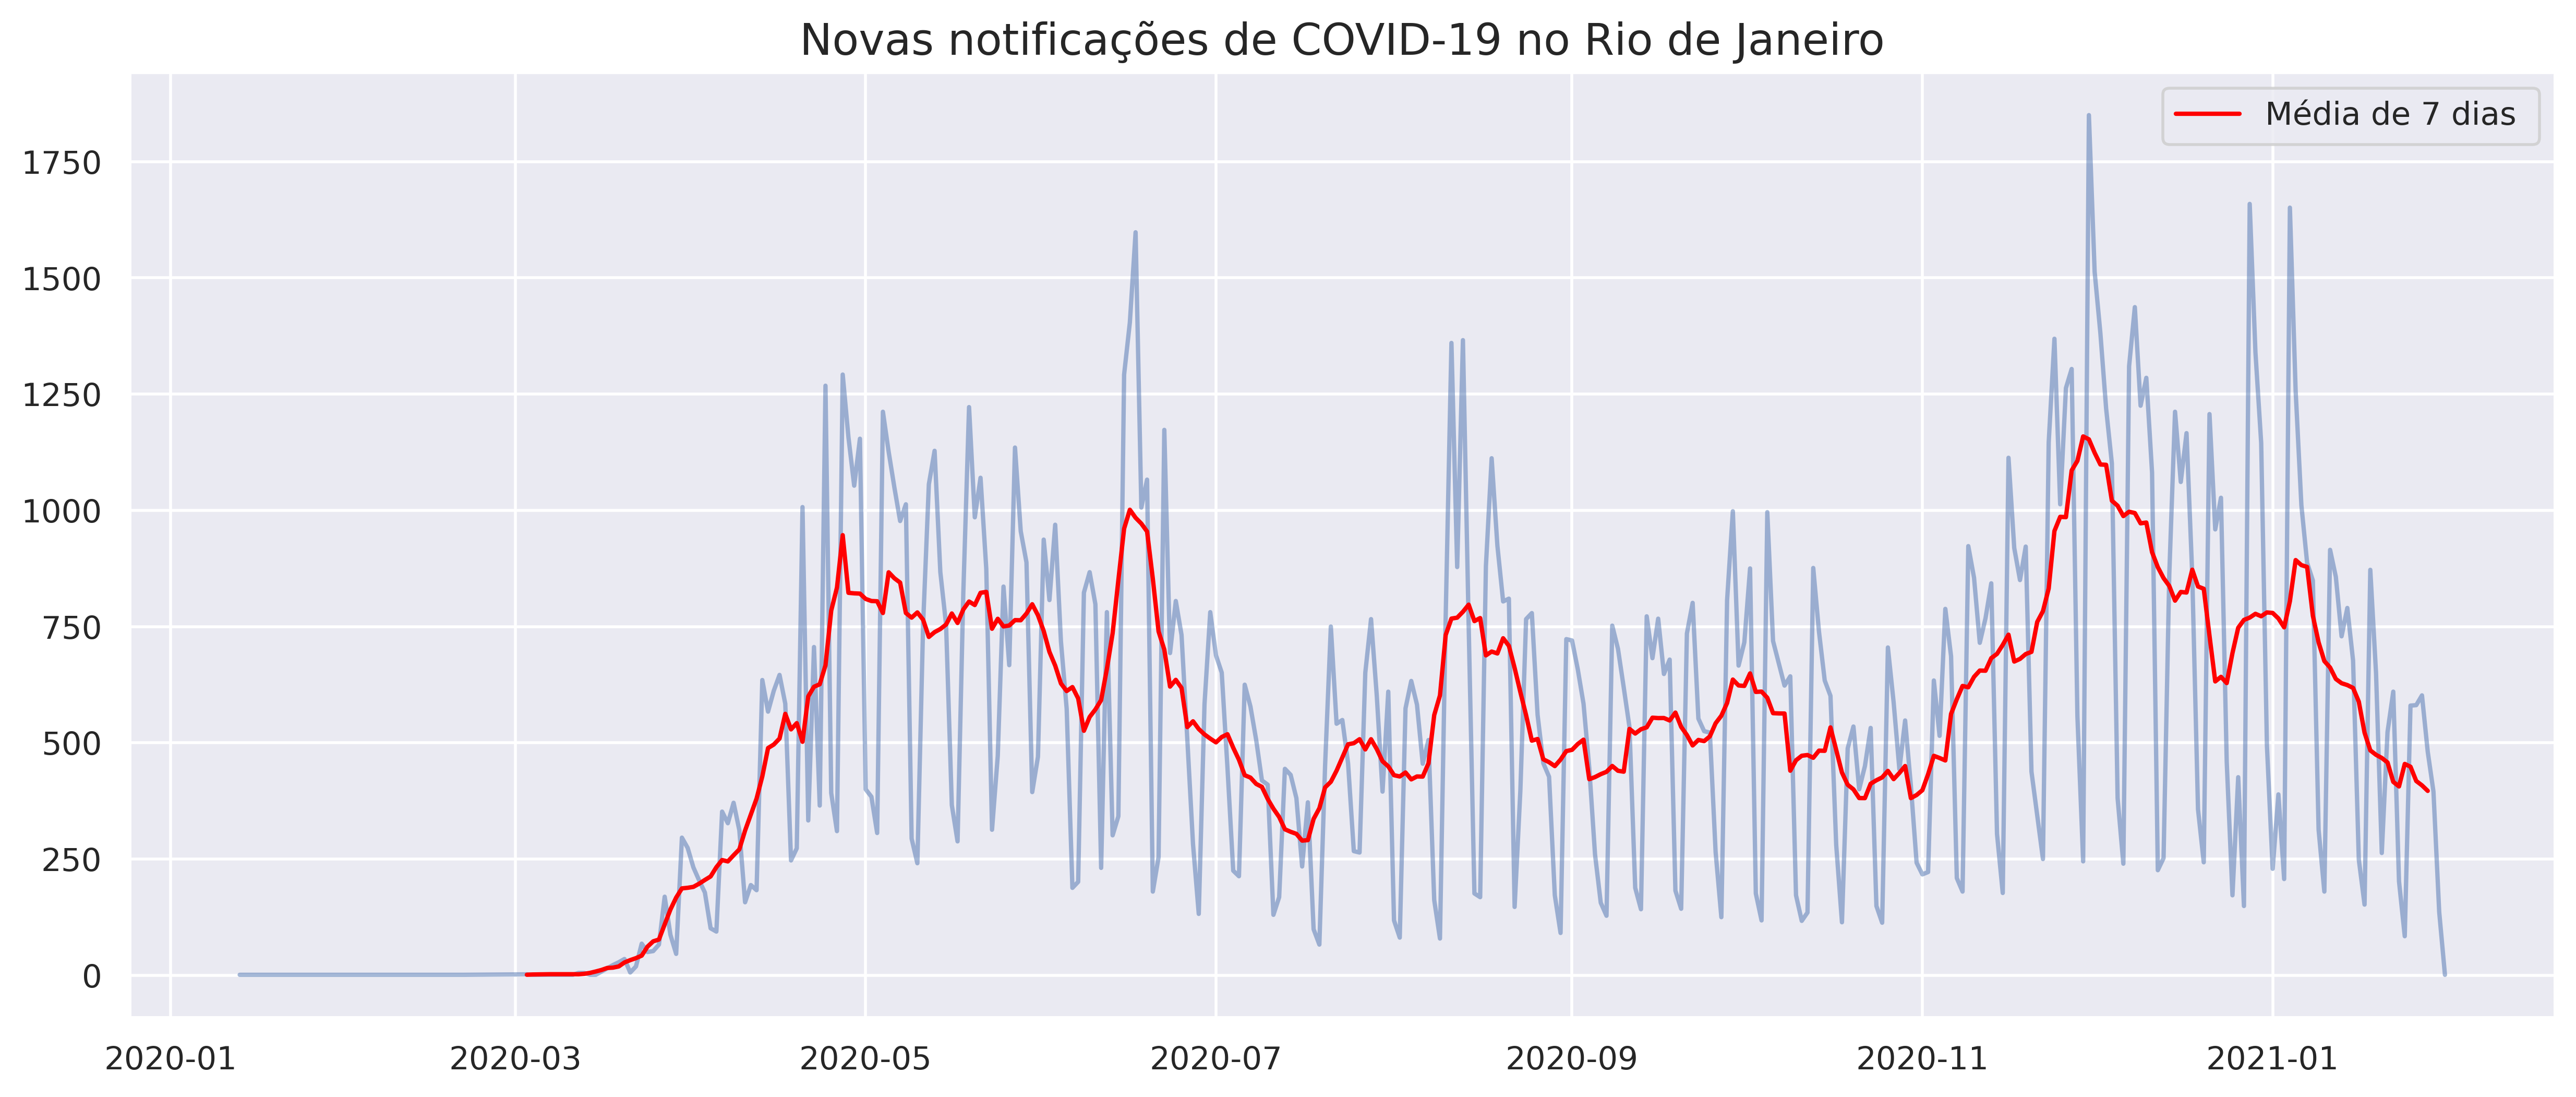
\includegraphics[width = \textwidth]
    {../images/new-notifications-rio.png}
    \caption{Notificações a cada dia ao longo da pandemia no Rio de Janeiro.}
    \label{new-notifications}
\end{figure}

\begin{figure}[!ht]
    \centering
    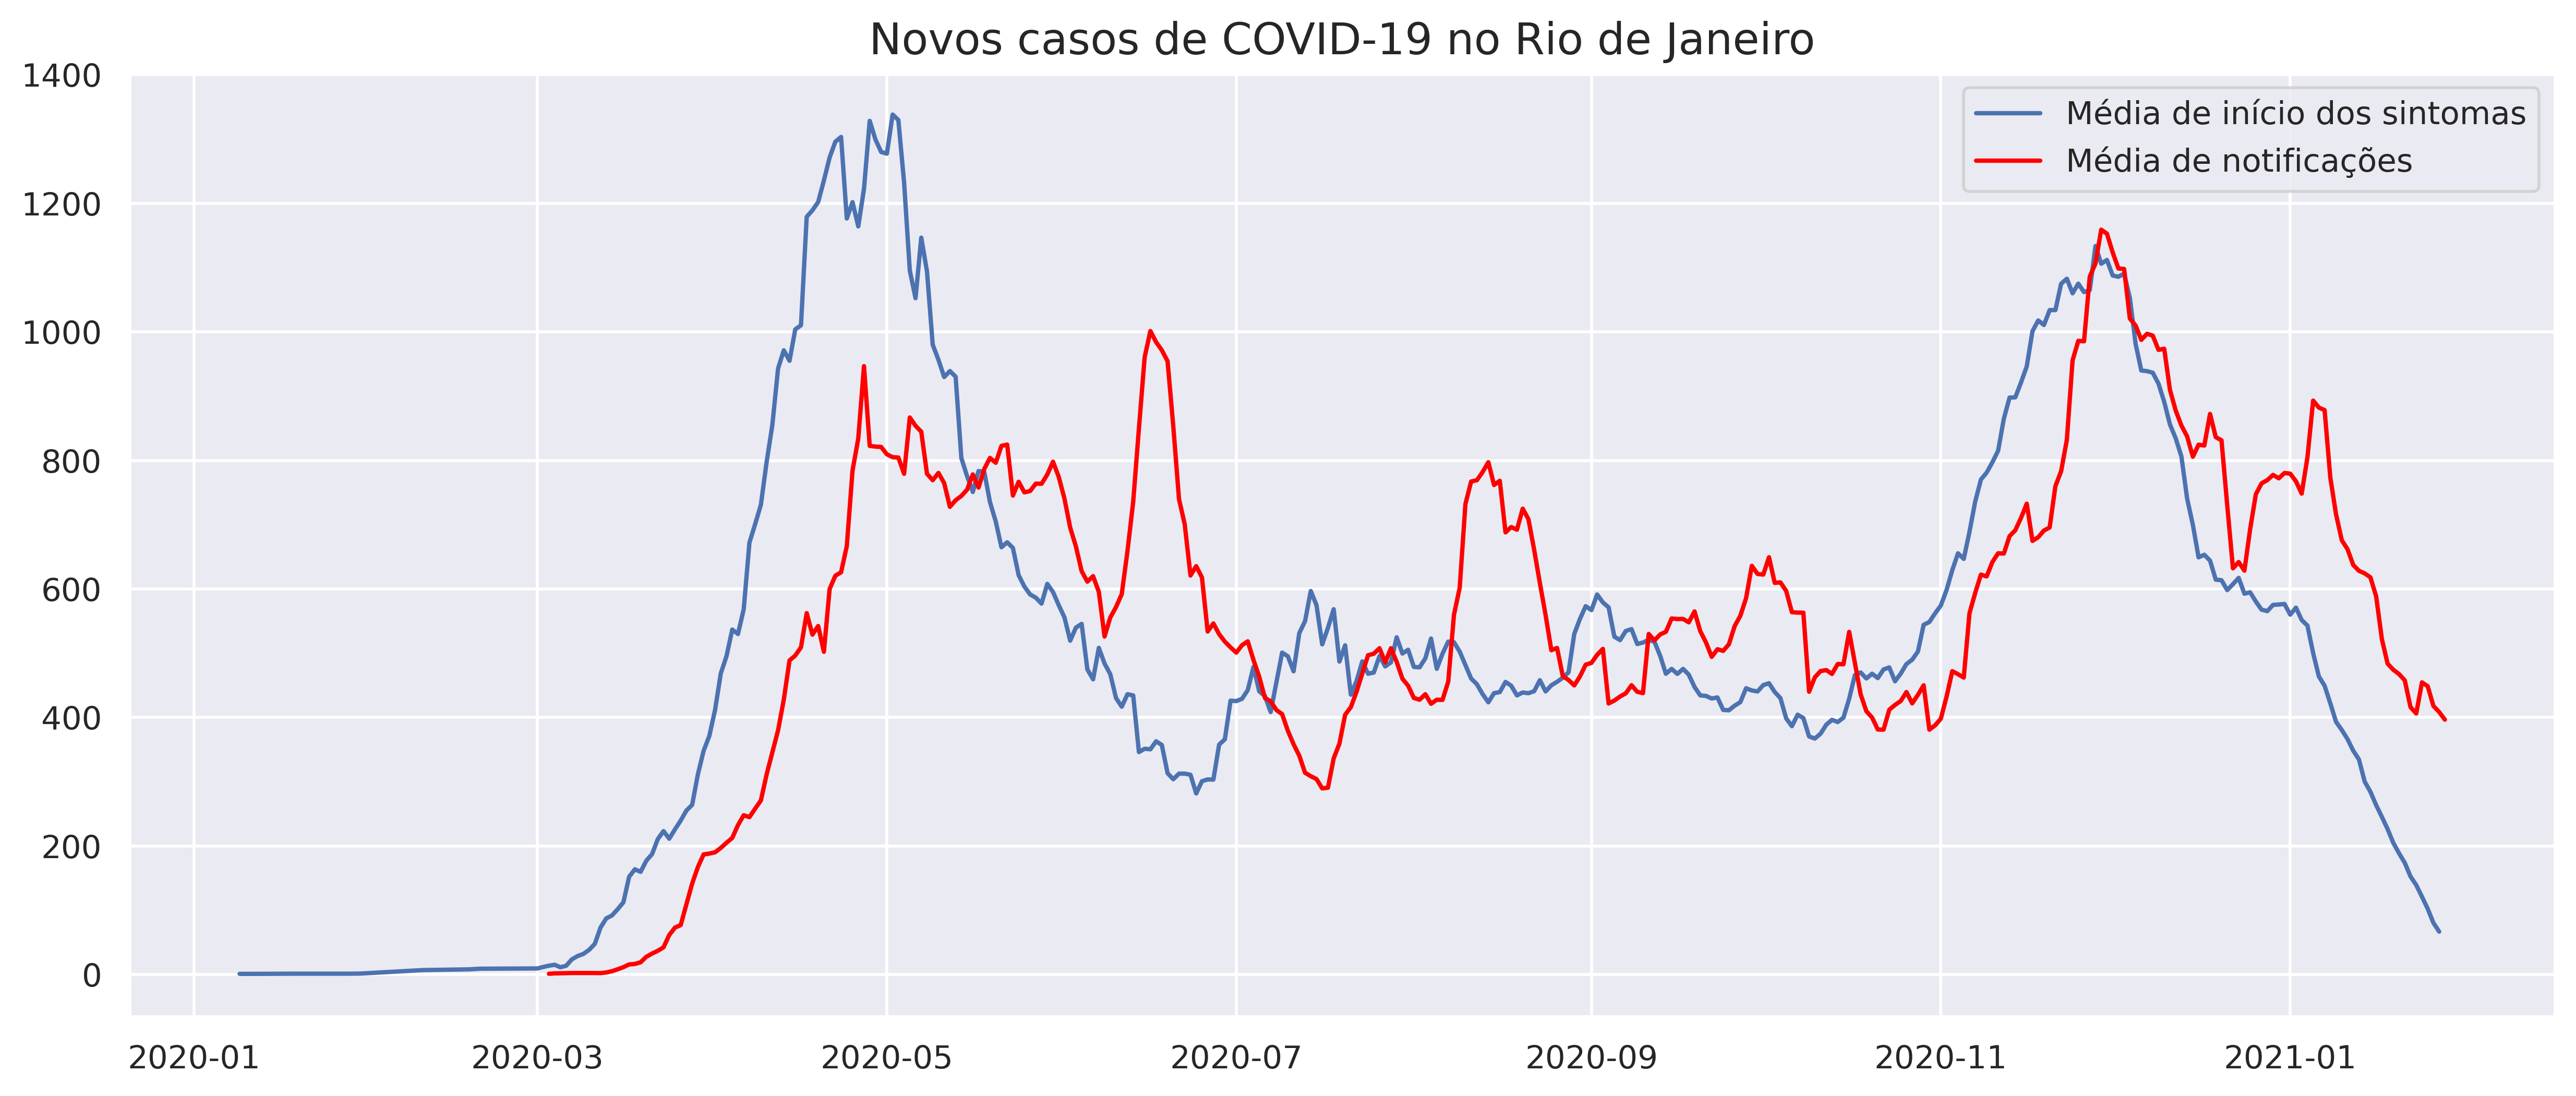
\includegraphics[width = \textwidth]{../images/comparing-symptoms-notifications.png}
    \caption{Comparação das curvas de média de 7 dias de novas notificações e indicação de início dos sintomas.}
    \label{notifications-vs-symptoms}
\end{figure}

Em agosto, o pico na média de notificações não é antecipado por um pico na curva de sintomas, isto é, as pessoas que notificaram esse mês devem ter começado a sentir os sintomas em um período anterior. 
Isso sugere que a curva em azul (média por início dos sintomas) é melhor a ser analisada, pois não sofre pelos problemas de atraso e inconstância. 
No final dessa curva, existe um decréscimo que não faz sentido com o pico anterior, pois as pessoas que indicarão o início dos sintomas nesse período vão ser notificadas nas semanas seguintes. 

Essa diferença de quando uma pessoa foi notificada e quando ela sentiu os primeiros sintomas pode ser visualizada em formato de histograma na Figura \ref{histogram-diff}. 
É importante destacar que valores negativos são claramente erros de digitação ou informação nos dados, como pôde ser examinado que existiam casos que foram notificados em 2021, mas com início dos sintomas em janeiro de 2020. 
Apesar disso, esses erros são em menor quantidade quando comparados à massa de dados. 
Registrou-se que em torno de 19,34\% dos dados têm tempo de notificação maior do que 30 dias e em torno de 1,29\% maior de 100 dias o que indica o grande atraso nas notificações.

\begin{figure}[!ht]
    \centering
    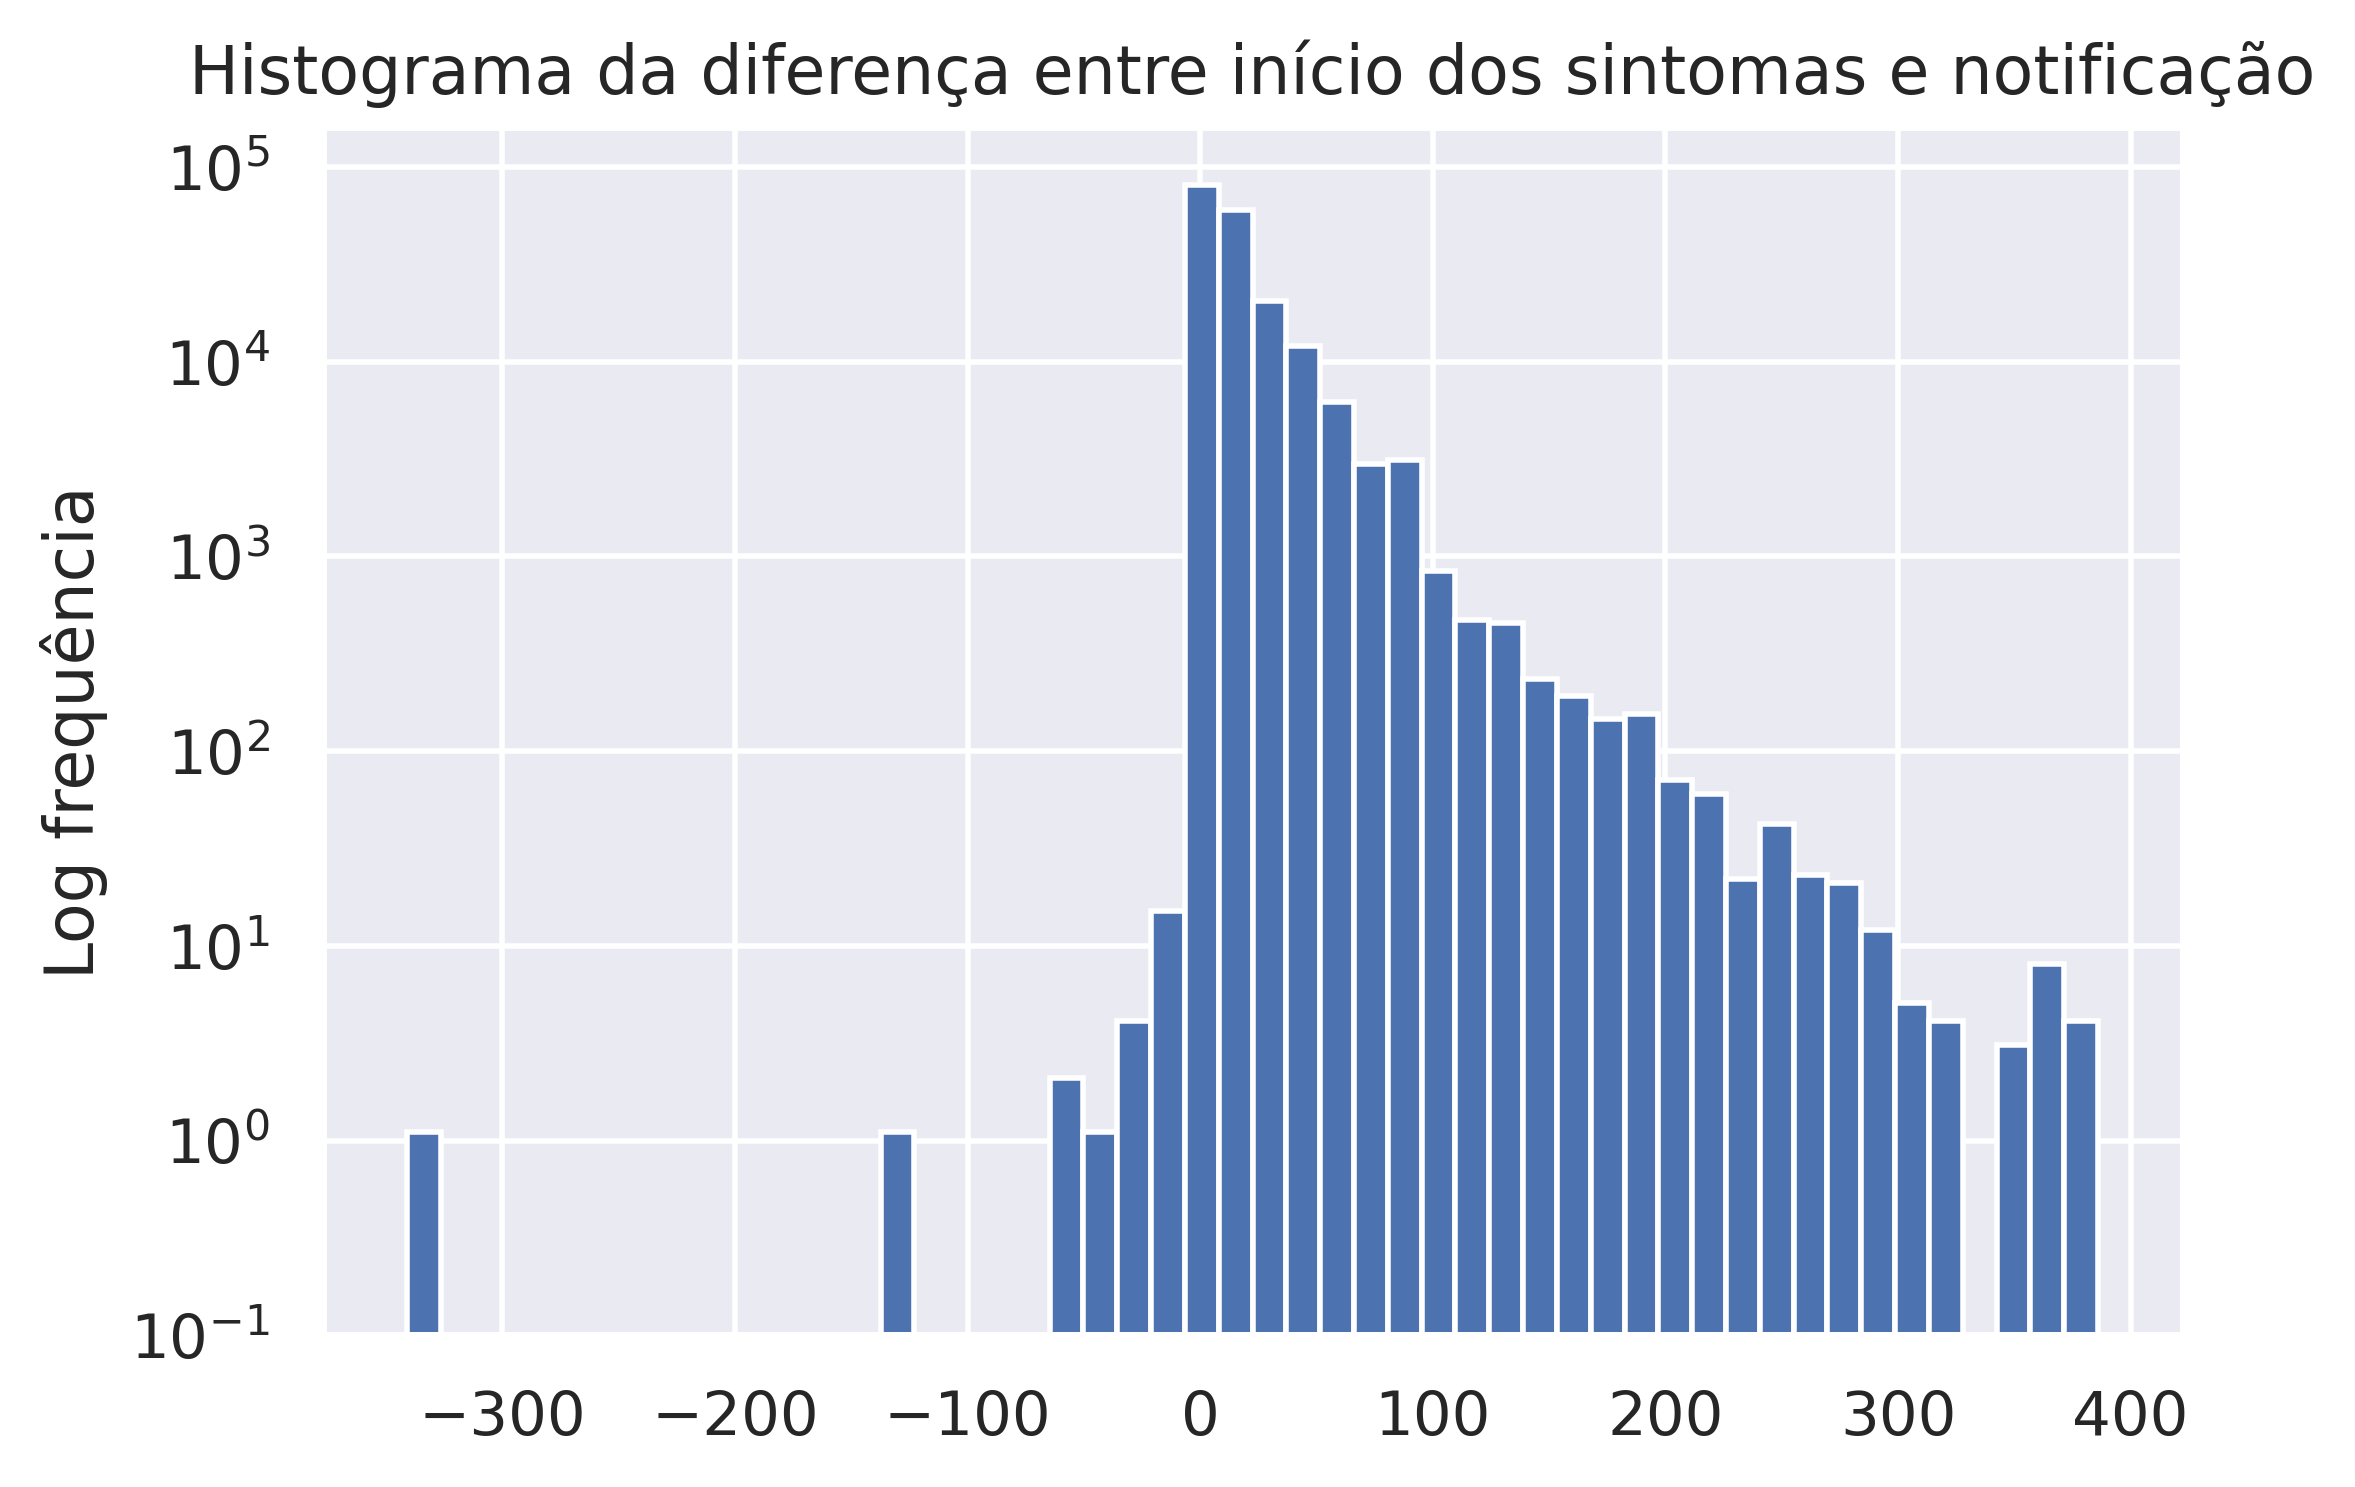
\includegraphics[width = .7\textwidth]{../images/histogram-comparion.png}
    \caption{Histograma da diferença entre o dia de notificação e o dia de início dos sintomas.}
    \label{histogram-diff}
\end{figure}

Uma análise com relação aos dados faltantes com comparação aos bairros, faixa etária e sexo também foi feita e pode ser vista no Github, mas apresentou pouca evidência para contribuir nesse trabalho. 
O mesmo tipo de exame pode ser feito para a evolução dos casos de óbitos, como pode ser visualizado na Figura \ref{deaths}. 
Muitos casos de mortes tiveram sua notificação a posteriori também, e omitimos o gráfico por razões de similaridade com o histograma anterior.
Por fim, para os campos com dados faltantes em data de início de sintomas e data de evolução daqueles com óbito registrado, houve uma imputação aleatória baseada na distribuição dos histogramas correspondentes. 

\begin{figure}[!ht]
    \centering
    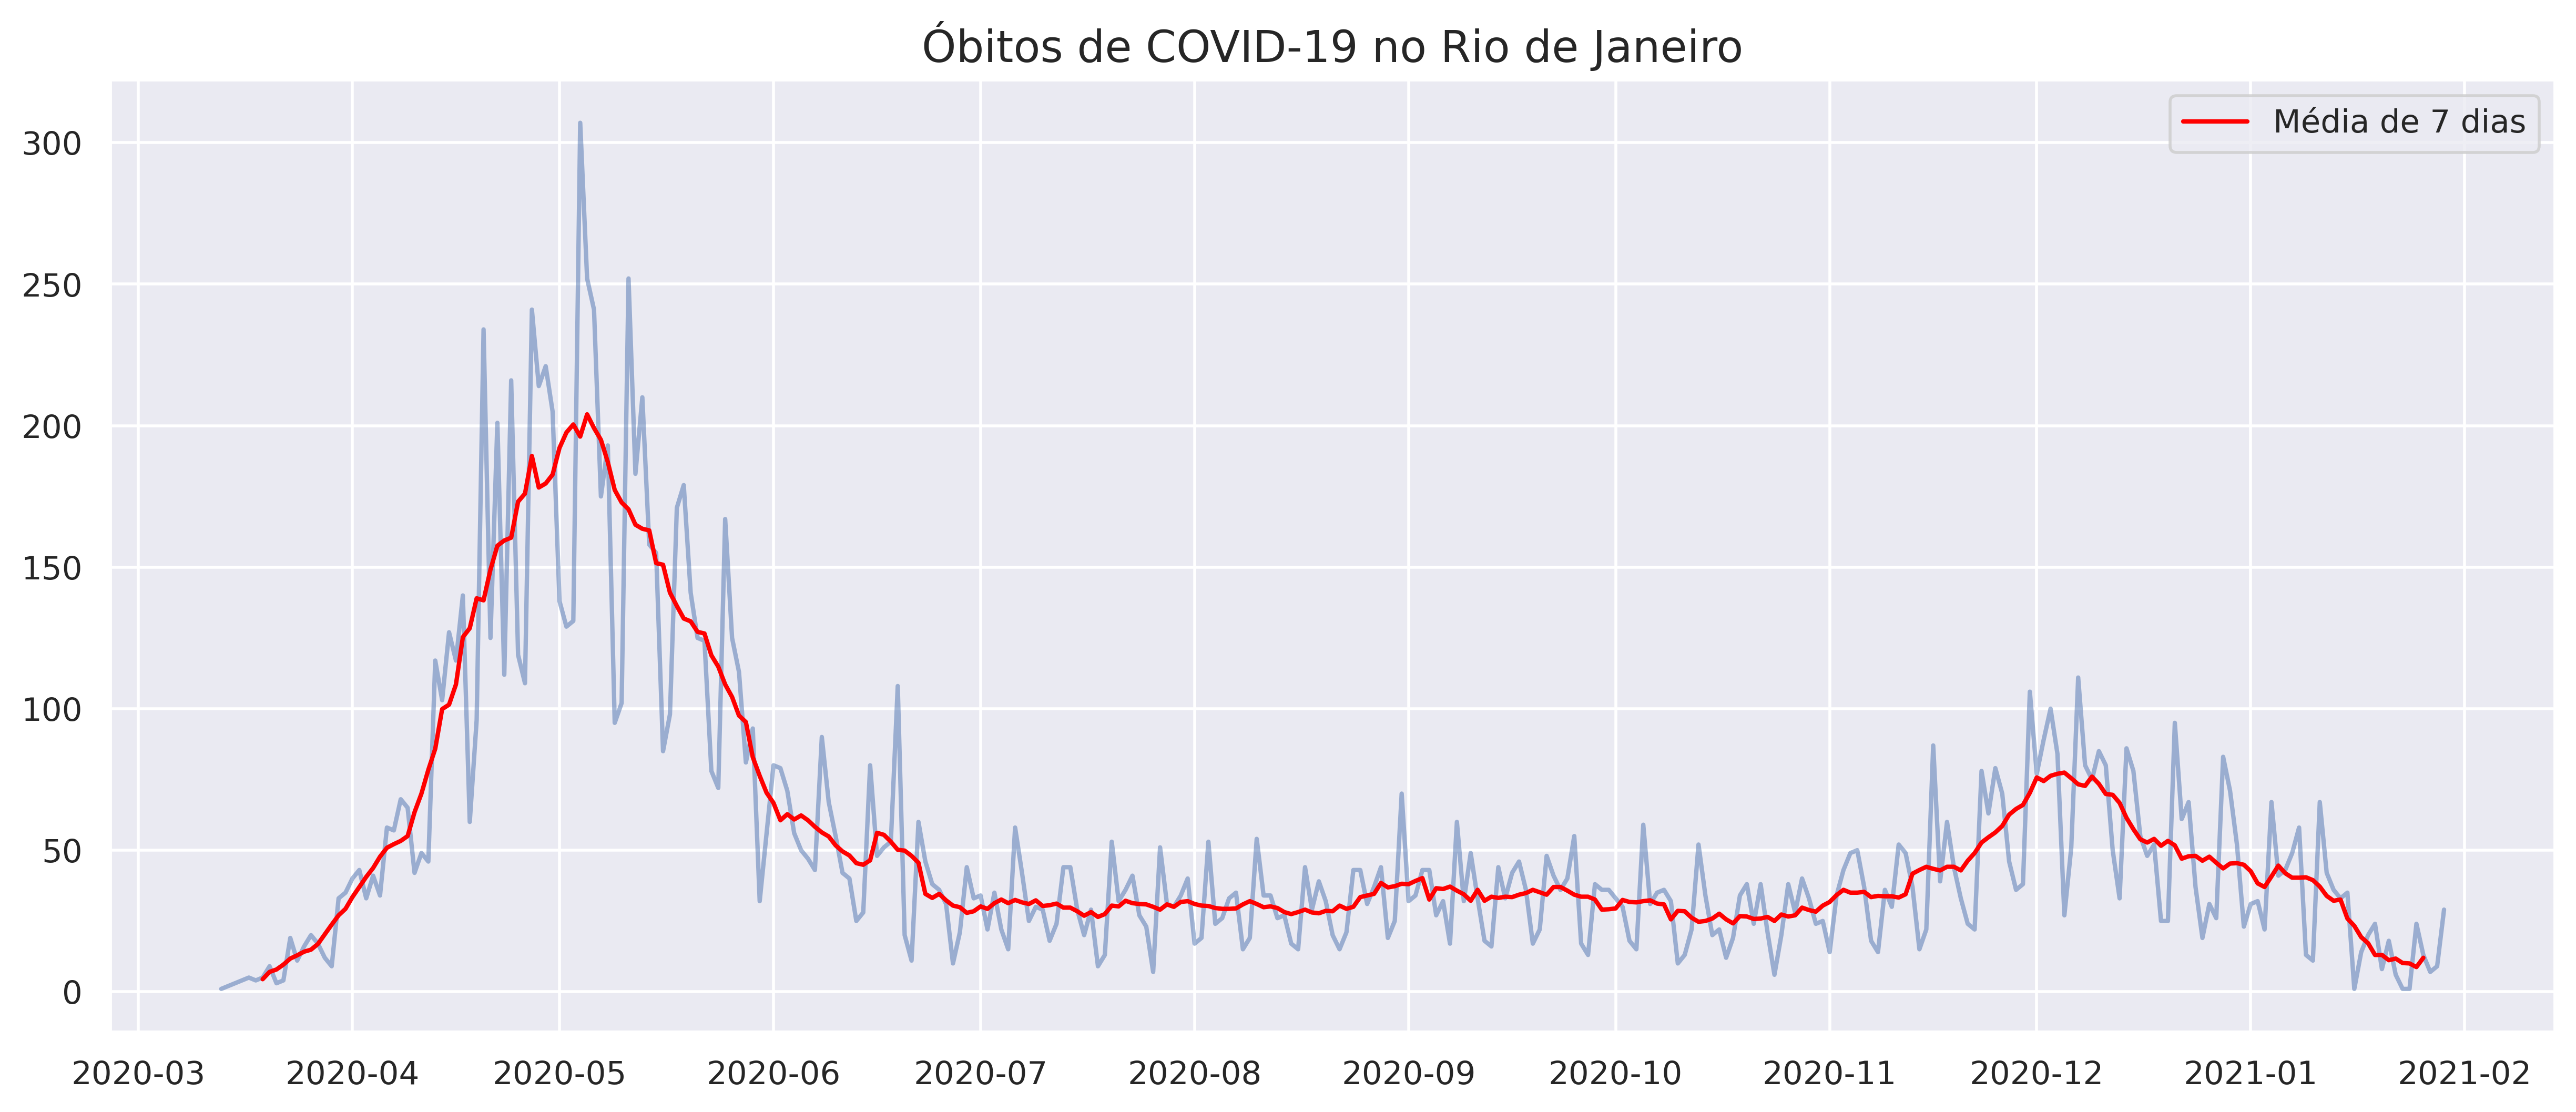
\includegraphics[width = \textwidth]{../images/deaths-rio.png}
    \caption{Evolução de óbitos no Rio de Janeiro.}
    \label{deaths}
\end{figure}

\subsection{Suavização das curvas}
\label{moving-average}

Constatamos ao longo do surto que existe uma sazonalidade semanal nos casos confirmados e de mortes, dado que nos fins de semana há um desvio negativo, enquanto na terça-feira um positivo. 
Essa variação semanal prejudica o modelo, pois ele não possui ajuste sazonal e, por esse razão, a aplicação de um suavizador se faz necessária. 
Nesse sentido, utilizaremos uma {\em média móvel} centrada com 7 dias.
Desta forma, se  $\{x_s\}_{1 \le s \le n}$ são nossos dados iniciais, estamos interessados em
\begin{equation}
    \hat{x}_t = \frac{1}{2k + 1}\sum_{s=-k}^k x_{t+s},
\end{equation}
em que $2k + 1 = 7$. Essa escolha é arbitrária, mas deriva diretamente da problemática semanal.

\subsection{Dados acumulados}

Por fim, obtemos as curvas acumuladas de novos casos e óbitos, a fim de
comparar com as curvas do modelo $T$ e $D$. Dessarte, nosso dado será da
forma
\begin{equation}
    y_t = \sum_{i=-14}^t \hat{x}_i, ~~~~(t = 0, ..., n)
\end{equation}

\section{Estimativa dos parâmetros}
\label{parameters}

A construção do método de estimação presente nesse trabalho foi baseada em \cite{cao2012, liang2010, ramsey2007}. 
Como explicitado na Seção \ref{data}, os dados representam a informação diária do número de casos novos e de mortes a partir do começo de março, sendo que o primeiro dia desse mês tem muito mais casos do que o esperado e, portanto, foi excluído da análise. 
Consideraremos o início do modelo sendo o dia 16, quando as primeiras medidas de contenção foram tomadas \cite{decreto-emergencia} e a evolução do vírus deixa de ser tão irregular.
No modelo, essas curvas são acumuladas [Seção  \ref{apresentation}] e, portanto, observamos 
\begin{align}
    \hat{x}^{(1)}_i = (T(i) - T(i-1)) + \varepsilon^{(1)}_i, i = -14, ..., n
    \label{obsT1}
    \\
    \hat{x}^{(2)}_i = (D(i) - D(i-1)) + \varepsilon^{(2)}_i, i = -14, ..., n
    \label{obsD1}
\end{align}
em que $\hat{x}_0^{(1)}$ se refere ao aumento do número de casos notificados no dia 16 de março e $n$ é o número de dias considerados. 
Assumimos que $\{\varepsilon^{(1)}_i\}_{-14 \le i \le n}$ e $\{\varepsilon^{(2)}_i\}_{-14 \le i \le n}$ são sequências de variáveis independentes e normalmente distribuídas com variâncias $\sigma_k^2, k = 1,2$ desconhecidas\footnote{A hipótese de normalidade tem a intuição de ser a soma de vários pequenos erros individuais independentes.}. 
Para facilitar, vamos trabalhar com as observações 
\begin{align}
    y^{(1)}_i = T(i) + \xi^{(1)}_i, i = 0, ..., n
    \label{obsT}
    \\
    y^{(2)}_i = D(i) + \xi^{(2)}_i, i = 0, ..., n
    \label{obsD}
\end{align}
onde, para $k=1,2$, definimos $\xi_i^{(k)} = \sum_{j=-14}^i
\varepsilon_j^{(k)}$. Se tormarmos $i \le j$, calculamos 
\begin{equation} 
    \label{cov-matrix}
    Cov(\xi_i^{(k)}, \xi_j^{(k)}) = (i + 15)\sigma_k^2
\end{equation}
e o vetor $\boldsymbol{\xi^{(k)}}$ tem distribuição normal multivariada com média 0 e matriz de covariância dada pela equação \eqref{cov-matrix}. 
Normalizarmos os dados obtidos pelo tamanho da população, que assumimos ser de 6.7 milhões \cite{ibge-rio} no Rio de Janeiro. 
A estimação dos parâmetros foi dividida em (1) identificabilidade, (2) ajuste nos dados e (3) quantificação da incerteza.

\subsection{Escolha e modelagem dos parâmetros}

Afirmamos que os parâmetros $\tau, \sigma, \gamma_1, \gamma_2$ e $\delta$ são epidemiológicos e, portanto, utilizamos estimativas da literatura que podem ser encontradas na Tabela \ref{tab:parameter_values}. 
O parâmetro de testagem $\rho$ é aproximado segundo a Observação \ref{estimativa-rho}. 
Por fim, os parâmetros $\beta(t), \alpha$ e $\mu(t)$ são estimados, de forma que a transmissibilidade e mortalidade são modeladas conforme explicado na Seção \ref{estimativa-beta}. 

\begin{table}[ht]
    \centering
    \begin{tabular}{|c|c|c|}
    \hline
     {\bf Par.} & {\bf Valor} & {\bf Referência} \\[0.5ex]
    \hline 
    $\omega^{-1}$ &  5.74 dias & \cite{incubation2020} \\
    \hline
    $\tau^{-1}$ & 3.69 dias & \cite{latent2020} \\
    \hline
    $\sigma^{-1}$ &  $\omega^{-1} - \tau^{-1}$ & \cite{latent2020} \\
    \hline
    $\gamma_1^{-1}$  & 7.5 dias & \cite{recovery2020} \\
    \hline
    $\gamma_2^{-1}$ & 13.4 dias & \cite{recovery2020} \\
    \hline
    $\delta$ & 0.01 &  \cite{delta2020} \\
    \hline
    \end{tabular}
    \caption{Valores dos parâmetros epidemiológicos estimados pela literatura.}
    \label{tab:parameter_values}
\end{table}

\begin{obs.}[Estimativa parâmetro $\rho$]
    \label{estimativa-rho}
    Vamos considerar $\rho(t) \equiv \rho$ e utilizamos os dados de testagem do estado do Rio de Janeiro obtidos pelo IBGE através do PNAD COVID-19
    \cite{ibge-pnad} como resumido na Tabela \ref{Tab:testing-rio}. 
    Em particular, percebemos que 2\% da população é testada por mês, e entre os testados, 20\% eram positivos. 
    Sabemos que parte dessa testagem ocorre em pessoas que foram identificadas pelo sistema com o aparecimento de sintomas e gostaríamos de separar entre esses e aqueles que não possuíam sintomas, o que infelizmente não é informado.
    Então, por dia, a proporção de 0,00013 da população foi testada, isto é, $\rho \le 1.3\cdot 10^{-4}$. 
    Tomaremos $\rho = 10^{-5}$ e uma análise da influência dessa escolha é
    feita na Tabela \ref{tab:range-parameters}.

    \begin{table}[ht]
        \centering
        \begin{tabular}{|c|c|c|c|c|}
        \hline
          & {\bf Julho} & {\bf Agosto}  & {\bf Setembro} & {\bf Outubro} \\[0.5ex]
        \hline
        Percentual (\%) & 6,8 & 8,6 & 10,2 & 11,9 \\
        \hline
        Percentual que testaram positivo (\%) & 1,2 & 1,5 & 1,9 & 2,4 \\
        \hline
        \end{tabular}
        \caption{Percentual de pessoas que fizeram
        algum teste para saber se estavam infectadas pelo SARS-CoV-2 no total da
        população. }
        \label{Tab:testing-rio}
    \end{table}
\end{obs.}

\subsubsection{Estimação dos parâmetros que variam com o tempo}
\label{estimativa-beta}

Na cidade, ao longo da epidemia, ocorreram diversas medidas de isolamento, como, por exemplo, a obrigatoriedade do uso de máscaras \cite{decreto-mascaras} e o sistema de bandeiras \cite{sistemas-bandeiras}.
Por consequência, a taxa de transmissibilidade da doença, o parâmetro $\beta$ do modelo, varia conforme a aceitação dessas medidas pela sociedade.
A modelagem em si da resposta da sociedade é bem complexa e não será estudada nesse texto.
Então selecionamos o uso da aproximação por {\em B-splines}, que pode ser expressa da seguinte forma: 
\begin{equation}
    \label{beta-b-splines}
    \beta(t) \approx \sum_{j=1}^s \beta_j B_{j,k}(t)
\end{equation}
onde $\beta_j$ são os coeficientes a ser estimados e $B_{j,k}(t)$ formam a base de funções de ordem $k$. 
Além disso, foi observado que ao estimar o modelo em questão, apesar da curva de novos casos ter bons resultados, a curva de mortes teve um comportamento diferente: ela apresentou um pico bem mais concentrado e uma subida e descida muito mais intensas que as previstas. 
Por esse motivo, tratamos $\mu = \mu(t)$ da mesma forma que $\beta$, mas com $r$ coeficientes. 

Definimos, portanto, o vetor de parâmetros a ser estimado $\theta = (\alpha, \beta_1, ..., \beta_s, \mu_1, ..., \mu_r)$ com $s+r+1$ parâmetros. 
Por hipótese assumiremos que os {\it knots}, pontos onde os polinômios se ligam, são igualmente espaçados. 
Poderíamos procurar os pontos ótimos conforme os momentos da epidemia em que a resposta do público foi modificada segundo às ações tomadas pelo poder público.

\subsection{Identificabilidade}
\label{identificability}
O primeiro passo após a concepção do modelo é analisar sua {\em identificabilidade}, porque a estimação pode variar dependendo de quando o problema é ou não bem-posto. 
De forma geral, essa análise identifica se os parâmetros desconhecidos podem ser estimados de forma única \cite{audoly2001, sarcomani2019}. 
Existem duas formas de fazer essa análise: a forma estrutural (a priori) e a forma prática (a posteriori). 
A primeira é uma propriedade teórica que reside na própria estrutura do modelo. Os parâmetros são {\em estruturalmente identificáveis} se eles podem ser unicamente estimados a partir do experimento desenvolvido e são chamados {\em localmente estruturalmente identificáveis} se essa característica é verificada em torno do ponto ótimo. 
A segunda é feita após o processo de ajuste de dados, quando outros problemas podem aparecer em relação ao ruído encontrado na informação. Em particular, utilizaremos a {\em matriz de correlação} dos parâmetros.

Conforme descrito em \cite{ljung1994}, considere um sistema dinâmico
\begin{equation}
    \begin{aligned}
        \Dot{x} &= f(x(t), \theta), &x(0) = x_0 \\
        y(t) &= h(x(t), \theta)
    \end{aligned}
\end{equation}
em que $x(t) \in \R^n, y(t) \in \R^m$ e $f$ e $h$ são vetores de funções racionais da variável $x$ e $\theta \in \Theta \subset \R^p$. 
A variável $y$ é observável e no nosso modelo é indicada pelos casos confirmados e mortes. 
Quando $x(0) = x_0$, denotamos $y = \psi_{x_0}(\theta, u)$ como a observação com esse valor inicial. 
O objetivo é contar o número de soluções da equação:
\begin{equation}
     \label{identificability-equation}
     \psi_{x_0}(\theta, u) =  \psi_{x_0}(\theta^*, u).
\end{equation}
Dizemos que esse modelo é {\em globalmente identificável} na solução $\theta ^*$ se a equação \eqref{identificability-equation} tem solução única $\theta = \theta^*$, para todo tempo $s$. 
Ele será {\em localmente identificável} se essa propriedade valer em uma vizinhança de $\theta ^*$. Aplicamos um método computacional de identificabilidade estrutural através do programa DAISY \cite{bellu2007}.

\subsubsection{DAISY - Differential Algebra for Identifiability of SYstems}

DAISY é um {\it software}, com base na linguagem de programação {\it Reduce},
específico para o problema de identificabilidade em sistemas dinâmicos, com
algumas condições brandas para a utilização. 
Se o modelo possui essas condições, a codificação e manuseio são fáceis, o que é
uma vantagem quando queremos aplicar os algoritmos algébricos envolvidos. 
Tratamos todos os parâmetros do modelo indicados na Seção \ref{apresentation} como
invariantes no tempo. 
Supondo o conhecimento da curva de recuperados $R$, o problema foi considerado
globalmente identificável. 
Infelizmente esses dados não são completamente disponíveis, conforme destacado
na Seção \ref{data-analysis} e na ausência deles,  o {\it software} não conseguiu
resolver em pelo menos 3 dias, e, portanto, decidimos não continuar por esse 
caminho. 
O código pode ser encontrado no Github \cite{github}.

\subsection{Ajuste nos dados}

\subsubsection{Hipóteses inicias}
\label{initial-hypotheses}

Vamos considerar que no início da epidemia $S \approx 1$. Com essa aproximação e restringindo o modelo para as equações de $E, I, A$ e $T$, temos um sistema com quatro equações lineares \eqref{initial-system}, cuja solução é combinação linear de exponenciais.  
Podemos assumir que a testagem diária no início da pandemia era de $\rho \approx 0$ e, como já mencionado na sessão anterior, os parâmetros $\gamma_1, \tau$ e $\sigma$ são conhecidos. Os parâmetros $\alpha$ e $\beta$ são fixos no período. 

\begin{equation}
    \begin{bmatrix}
        \dot{E} \\ \dot{I} \\ \dot{A} \\ \dot{T} 
    \end{bmatrix} = 
    \begin{bmatrix}
        - \tau & \beta & \beta & 0 \\
        \tau & -\sigma & 0 & 0 \\
        0 & \sigma \alpha & -\gamma_1 & 0 \\
        0 & \sigma (1 - \alpha) & 0 & 0  
    \end{bmatrix}\cdot
    \begin{bmatrix}
        E \\ I \\ A \\ T 
    \end{bmatrix} 
    \label{initial-system}
\end{equation}

O valor $T(-14)$ corresponde aos dados de confirmados em 2 de março e $T(-15) = 0$.  
Assim estimamos $\theta_0 = (\alpha, \beta, E(-14), I(-14), A(-14))$ de forma a minimizar a expressão pgf
\begin{equation}
    \sum_{i=-14}^{0} w_i\left(y_i^{(1)} - \hat{T}(i, \theta_0)\right)^2,
\end{equation}
em que $w_i = \dfrac{i+14}{14}$. Com essas estimativas, obtemos os valores $(E(0), I(0), A(0))$ que determinam o início da pandemia. 
Não há mortes no início da pandemia, o que permite colocar $\mu = 0$. 
Usando que $R(-14) = 0$, obteremos que $Q(-14) = T(-14)$ e, assim, podemos integrar as curvas $Q$ e $R$ até obter os valores $Q(0)$ e $R(0)$. 
Por fim $S(0) = 1 - E(0) - I(0) - A(0) - Q(0) - R(0)$.

\subsubsection{Método de estimação}
\label{estimation-method}

Utilizaremos o método de {\em mínimos quadrados ponderados} para estimar os parâmetros desconhecidos, considerando a observação de casos confirmados e mortes diárias como indicado nas equações \eqref{obsT} e \eqref{obsD}. 
Nessa abordagem, resolvemos um problema de minimização não linear com restrições e a cada iteração integramos o sistema de equações diferenciais. Definimos a função objetivo como:
\begin{gather}
\label{objective}
    F(\theta) = (y^{(1)} - \hat{T}(\theta))^T\Sigma^{-1}(y^{(1)} - \hat{T}(\theta)) + \psi(y^{(2)} - \hat{T}(\theta))^T\Sigma^{-1}(y^{(2)} - \hat{D}(\theta)) 
\end{gather}
tal que $\hat{T}(\theta)$ e $\hat{D}(\theta)$ são os vetores soluções
numéricas das equações diferenciais através do método Runge-Kutta,
$\sigma_k^2\Sigma$ é a matriz de covariância dada pela equação
\eqref{cov-matrix} ($k=1,2$) e $\psi$ é um peso de importância das mortes na
minimização e está relacionado à razão das variâncias $\sigma_1^2/\sigma_2^2$.
A escolha dessa função está relacionada com as propriedades estatísticas dos
dados. Sabemos que, pela hipótese de normalidade, minimizar a
expressão \ref{objective} é equivalente a maximizar a verossimilhança. 
Utilizamos o algoritmo L-BFGS-B \cite{byrd1995}, baseado no método de projeção gradiente e no algoritmo BFGS com uso limitado de memória computacional, implementado na biblioteca Scipy \cite{scipy} da linguagem de programação Python e o código está disponível no Github \cite{github}. 

\subsubsection{Análise residual e \texorpdfstring{$\mathcal{R}_t$}{Rt}
estimado}
\label{residual-analysis}

Escolhemos, de modo arbitrário, fixar a data final para análise dos dados em 31 de julho de 2020 e primeiro ajustamos a curva aos dias iniciais da epidemia, conforme explicado na Seção \ref{initial-hypotheses}. 
Obtemos o resultado na Figura \ref{Fig:initial-values}. 
Definindo a priori $\psi = 119.57$ (valor aproximado entre as variâncias dos dados de casos e óbitos) e os hiperparâmetros ligados à otimização, como os limites superior e inferior e chutes iniciais de cada parâmetro, vamos analisar os resíduos do ajuste de dados e o $\mathcal{R}_t$ induzido pela estimação dos parâmetros segundo: 
\begin{enumerate}
    \item[(i)] o número de coeficientes a serem estimados para $\beta$ e $\mu$; e 
    \item[(ii)] a ordem das B-splines para os parâmetros $\beta$ e $\mu$.
\end{enumerate}

\begin{figure}
    \centering
    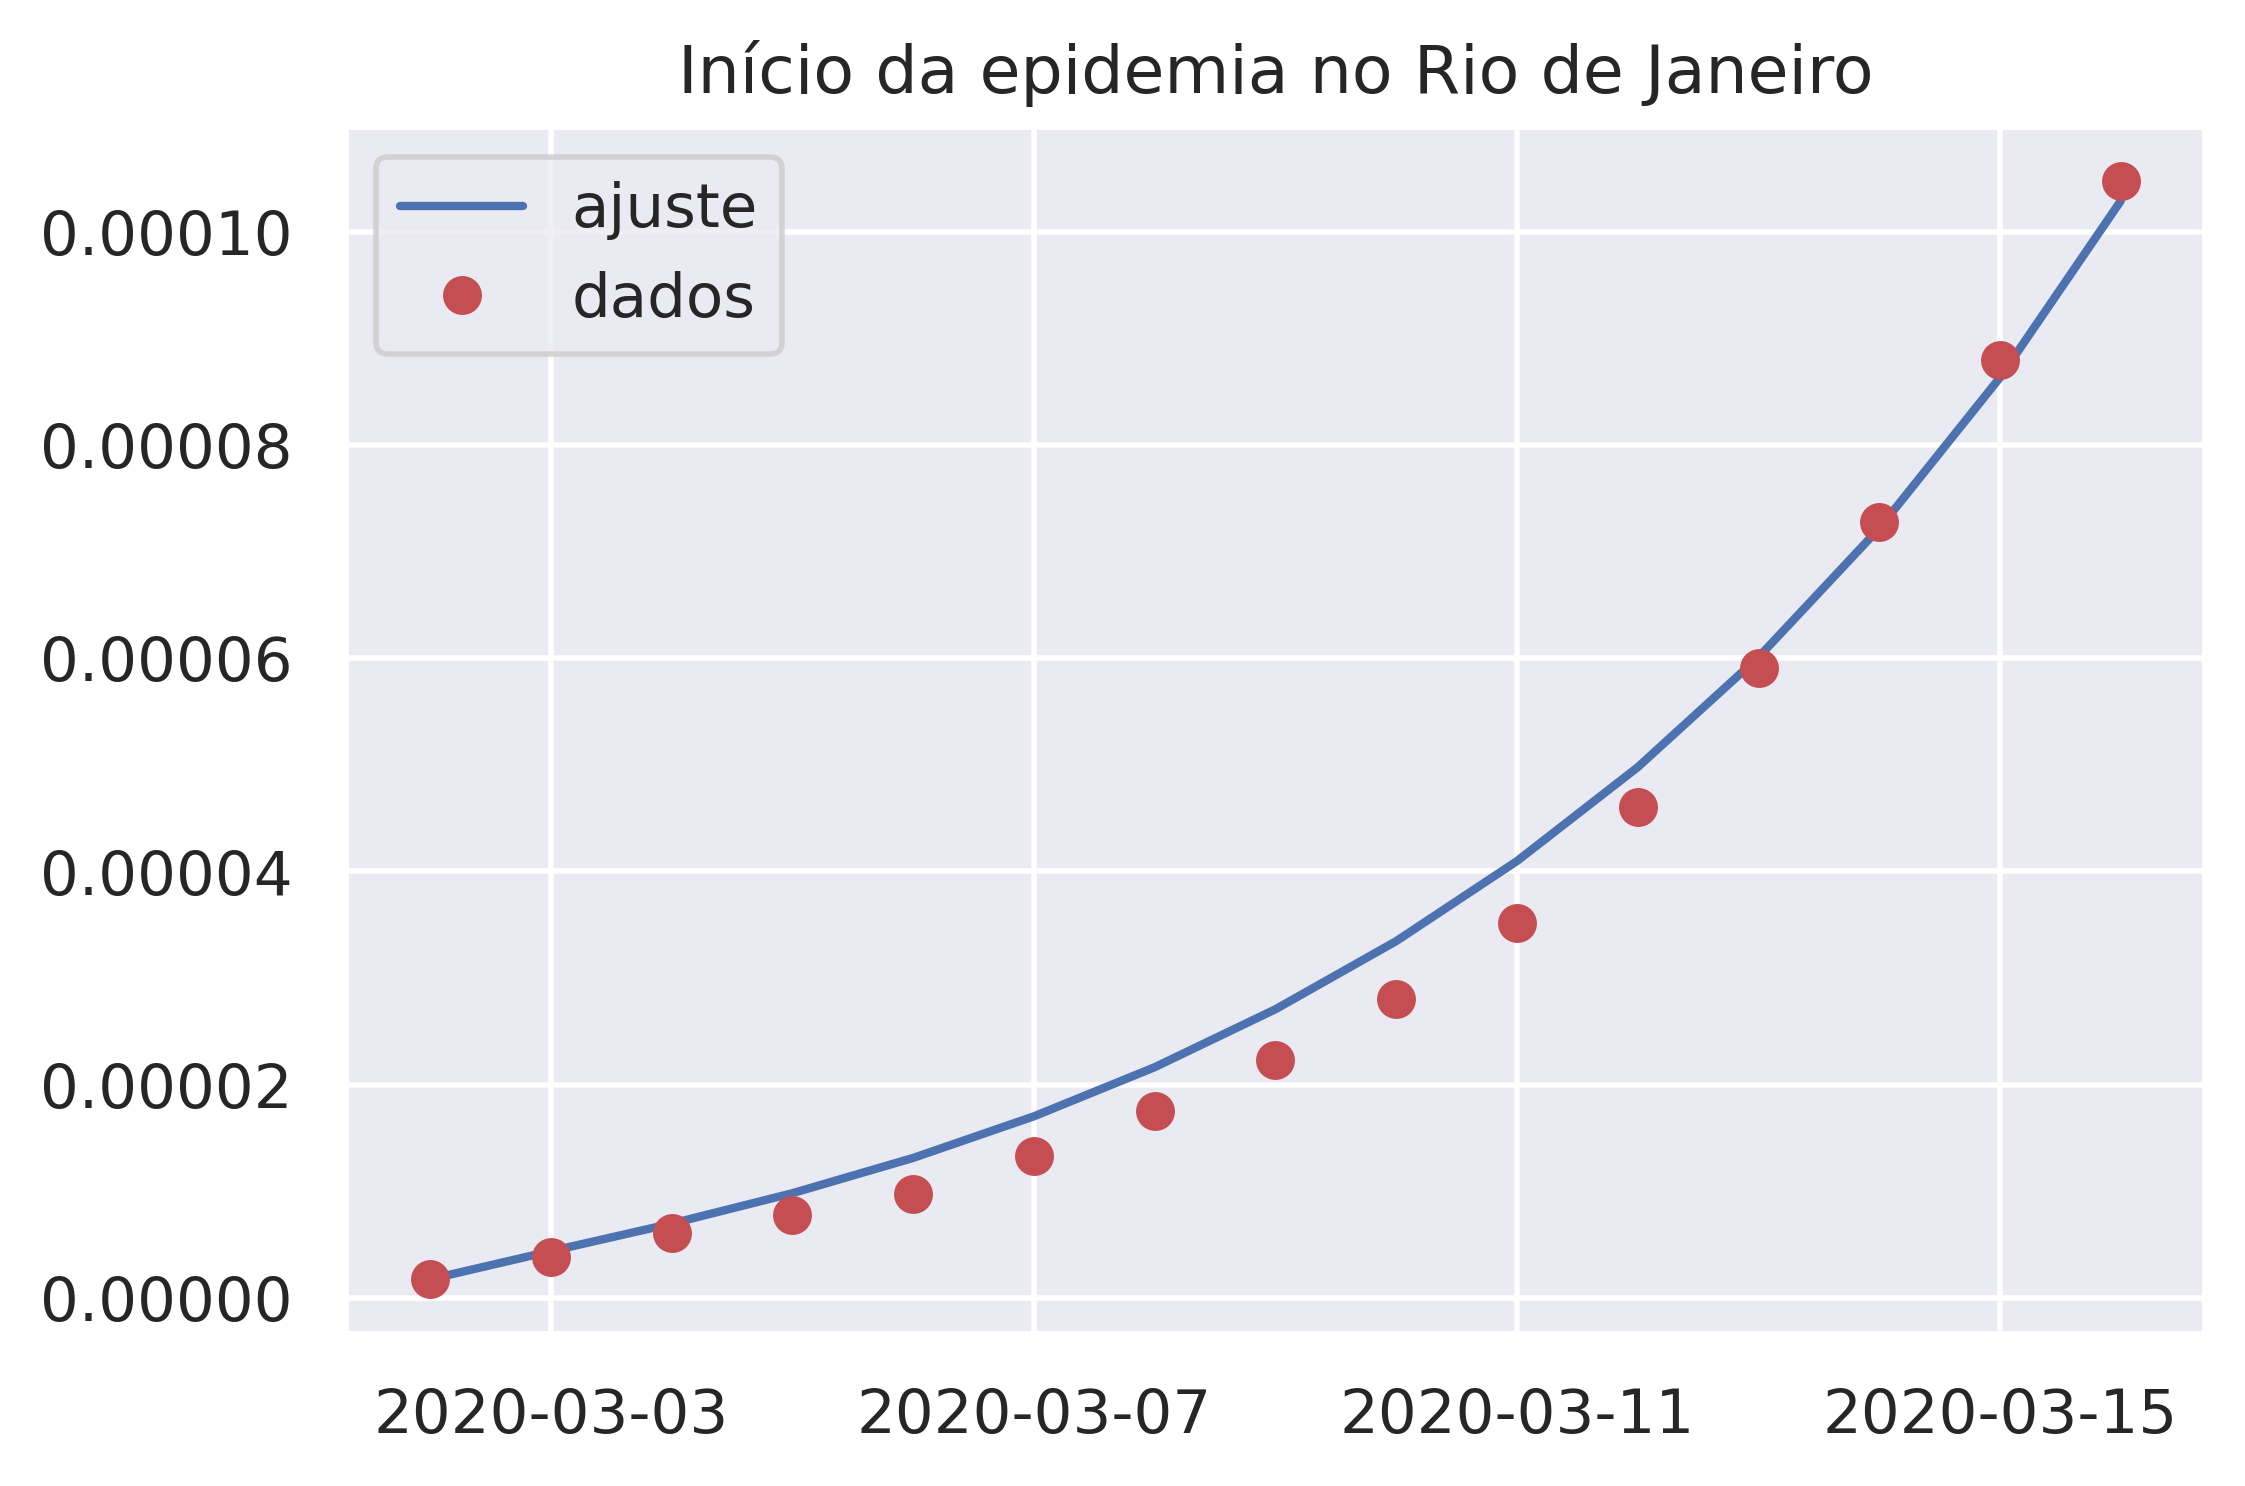
\includegraphics[width=0.5\textwidth]{../images/initial_values.png}
    \caption{Ajuste à curva acumulada de casos no início da epidemia para obtenção dos valores iniciais, como explicado na Seção \ref{initial-hypotheses}.}
    \label{Fig:initial-values}
\end{figure}

Por exemplo, colocando 4 coeficientes para as B-splines de ordem 3 para ambos
os parâmetros que variam no tempo, obtemos as curvas
descritas na Figura \ref{Fig:cumulated-curves}. Em particular $\alpha$ foi estimado em 0.899. 

\begin{figure}[H]
    \centering
    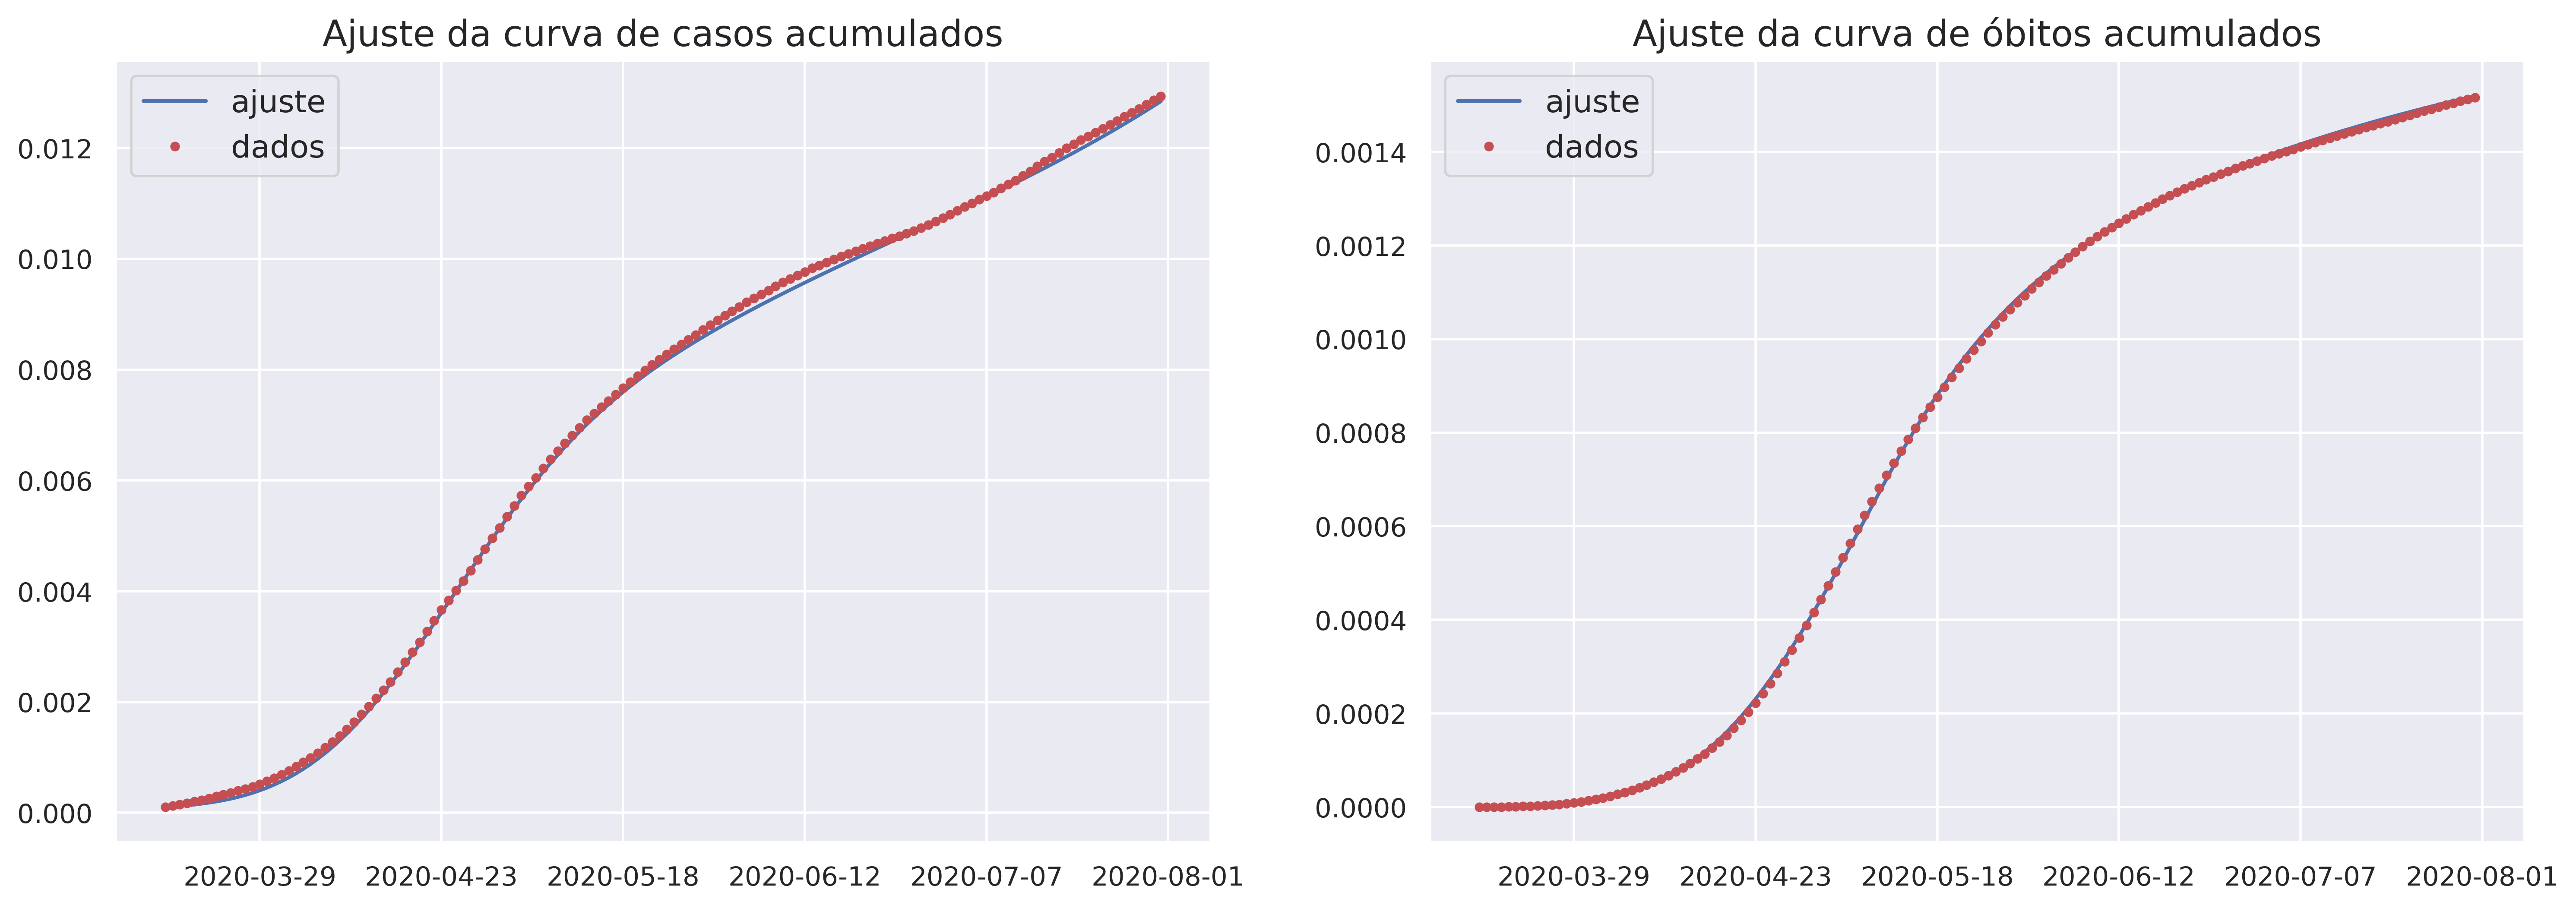
\includegraphics[width=\textwidth]{../images/cumulated_fitted_curves.png}
    \caption{Ajuste das curvas acumuladas de casos e óbitos, respectivamente.}
    \label{Fig:cumulated-curves}
\end{figure}

Com esse resultado, podemos verificar se os resíduos do modelo aproximam os erros, que por hipótese têm distribuição Gaussiana. 
Primeiro diferenciamos para obter resíduos diários, de forma que sua variância seja constante (ver equações \eqref{obsT1} e \eqref{obsD1}) e, então, desenhamos os {\em histogramas} (indicador da frequência de cada resíduo) e os {\em gráficos Q-Q} (comparação dos quartis da distribuição Gaussiana com os quartis da distribuição amostral dos resíduos) que são apresentados na Figura
\ref{Fig:check_residuals}. 
Já visualizamos que ambas as curvas não têm um ajuste com resíduos como esperado, principalmente a curva de mortes. 
Além dessa análise visual, também podemos aplicar testes estatísticos  para verificar correlação e normalidade.  

O {\em teste Ljung-Box} \cite{ljung1978} é um teste estatístico que verifica a autocorrelação em uma série temporal, cuja hipótese nula afirma que as k-correlações são nulas, isto é, a série temporal é independentemente distribuída. 
Aplicando-o nos resíduos do ajuste para as duas curvas, obtivemos o p-valor 0 computacional, o que indica que os resíduos não são descorrelacionamos como assumimos. 
Já o {\em teste Jarque-Bera} \cite{jarque1980} avalia a assimetria e a curtose da distribuição amostral e compara com as da normal.
No nosso caso, a hipótese nula não foi rejeitada à nível 5\%, o que é um bom indicativo de normalidade dos resíduos. 
Concluímos, em particular, que o modelo, apesar de um ajuste interessante, com resíduos normalmente distribuídos, tem resíduos correlacionados, o que precisa ser melhor estudado em trabalhos futuros. 
Podemos fazer essa análise para todas as combinações de parâmetros que desejarmos. 
Para mais detalhes, confira no Github \cite{github}.

\begin{figure}
    \centering
    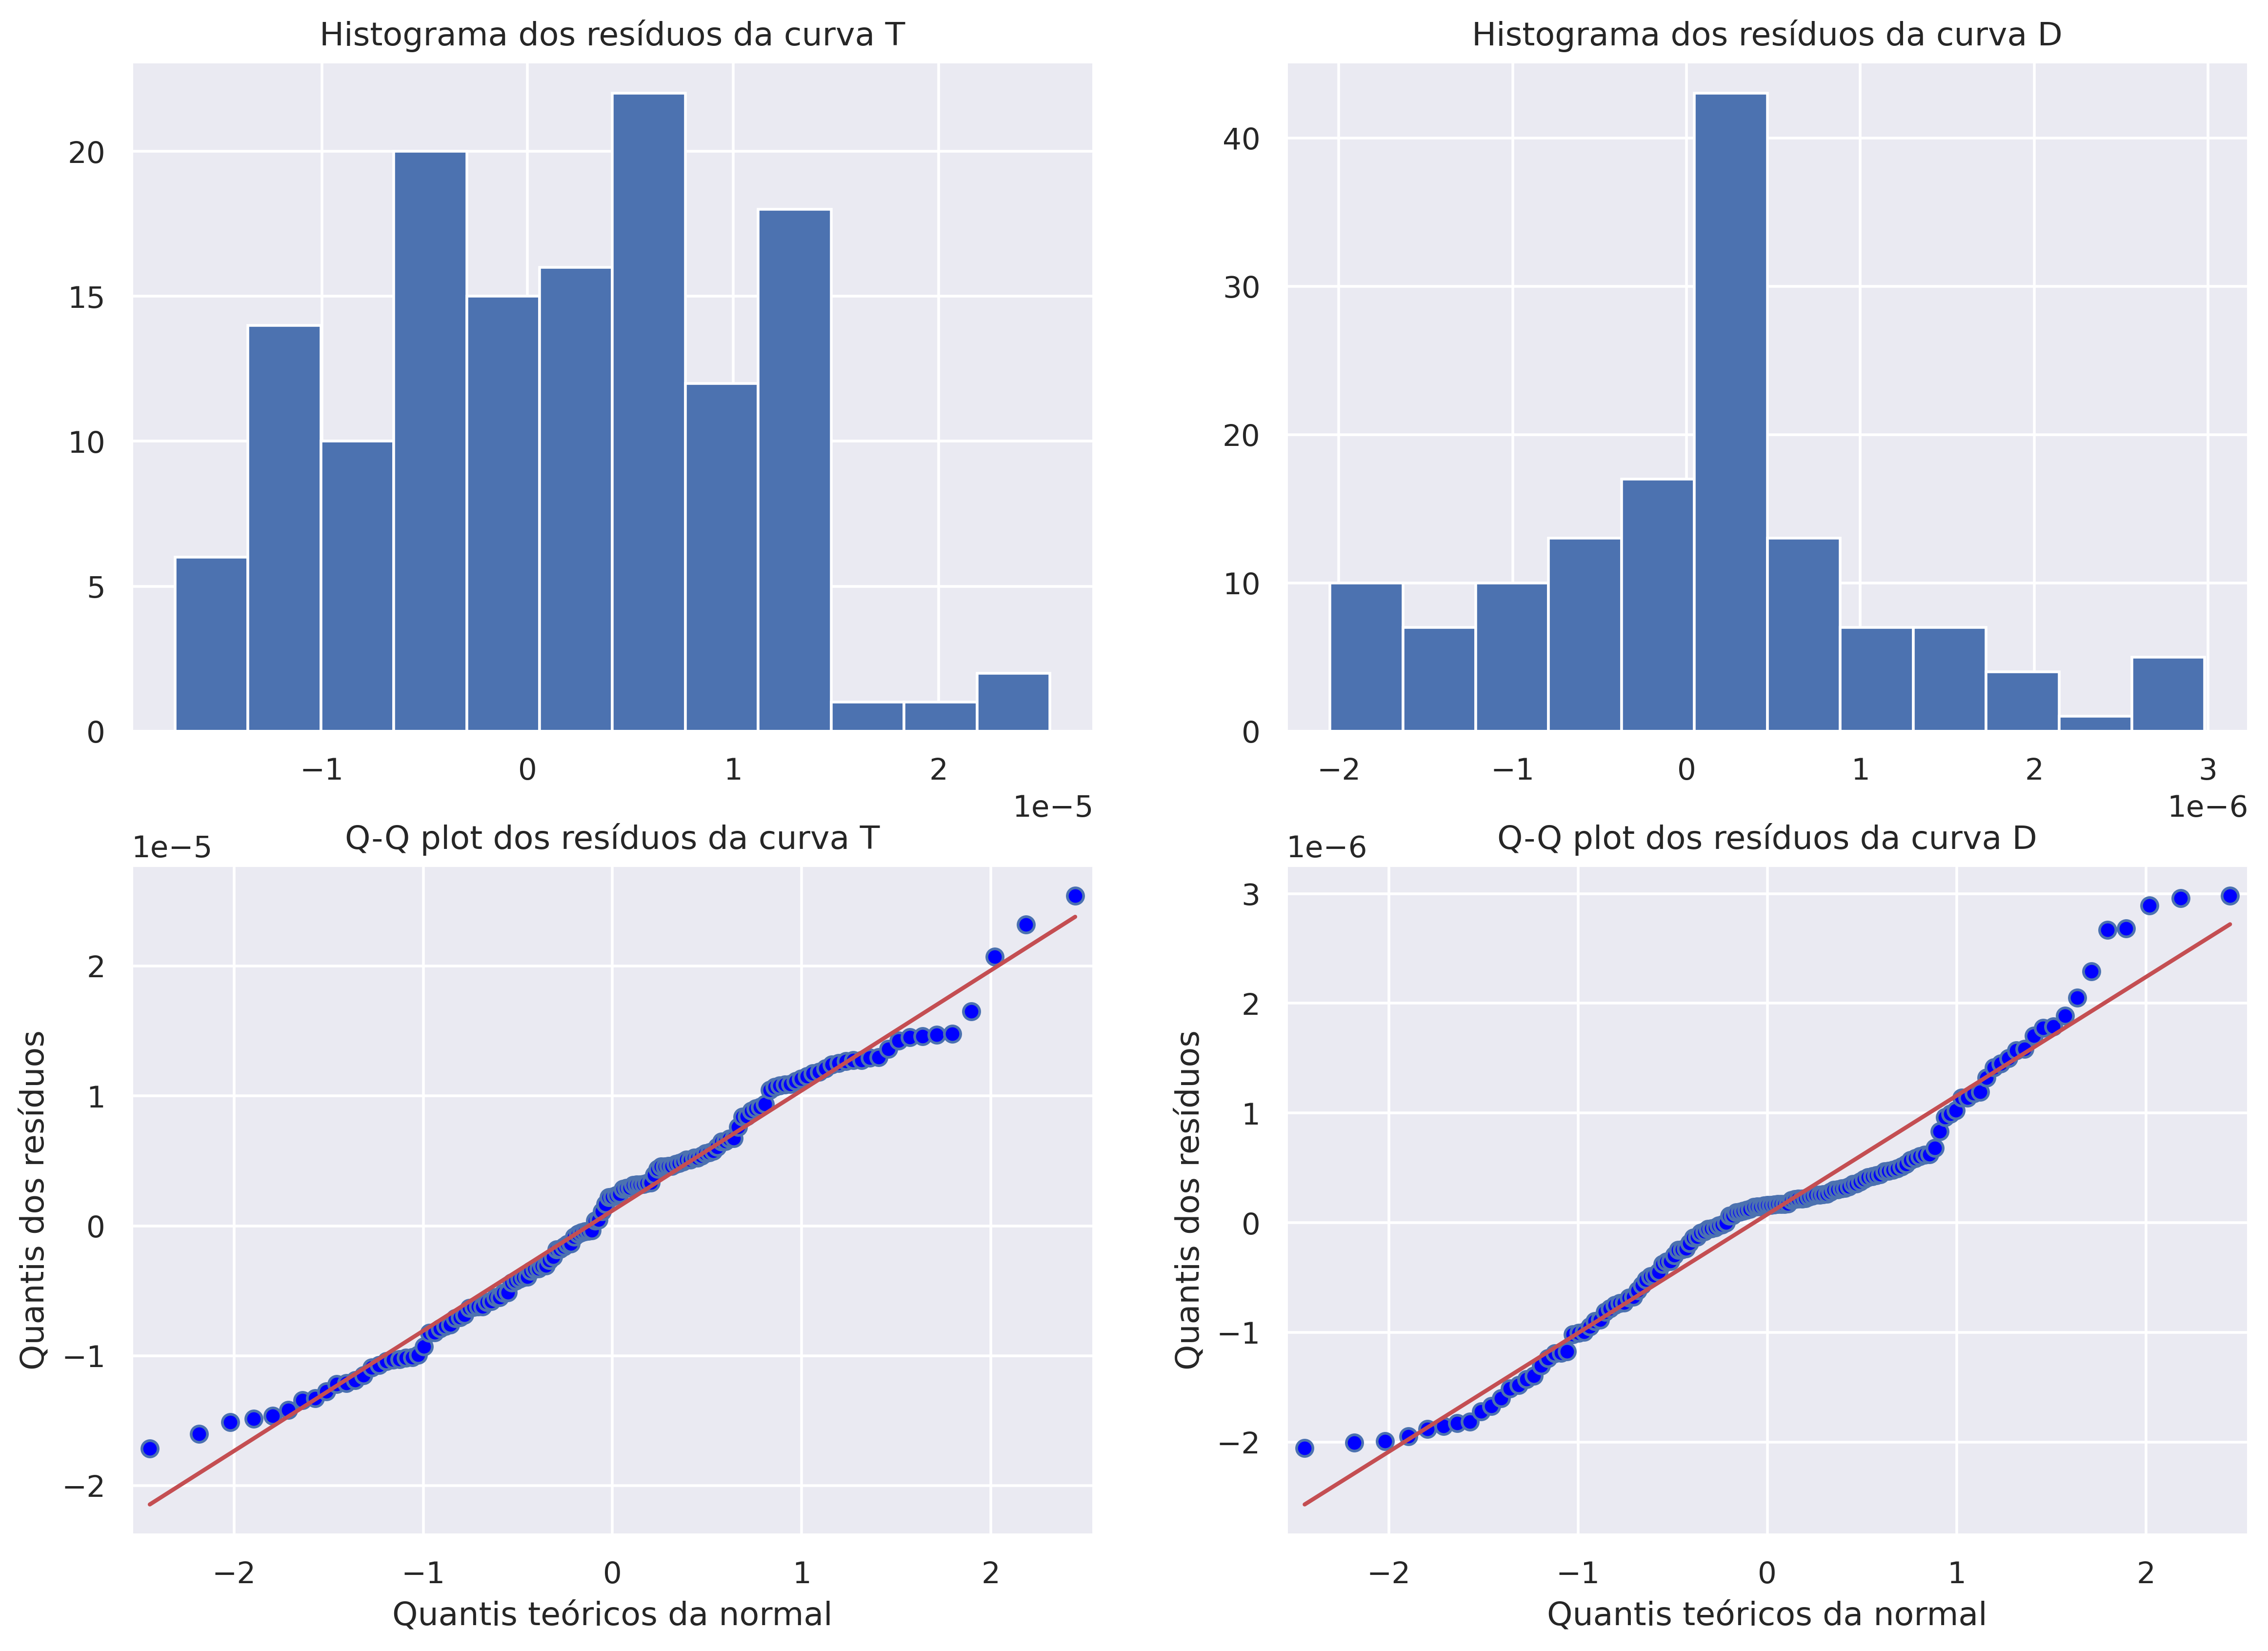
\includegraphics[width=.8\textwidth]{../images/check_residuals.png}
    \caption{Análise gráfica dos resíduos com histograma e Q-Q plot.}
    \label{Fig:check_residuals}
\end{figure}

Outra característica importante a ser analisada é o número reprodutivo básico,
descrito na Seção \ref{sec:R0}. Para os parâmetros estimados no exemplo,
obtemos o $\mathcal{R}_t$ descrito na Figura \ref{Fig:rt_modelo}. 
Considerando as estimativas do $\mathcal{R}_0$ para o Brasil em
\cite{rtBrasil2020}, encontramos no dia 23 de março o valor de 2.325
para o modelo SIRD, e 2.897 para o modelo SIRASD. Em
\cite{rt-imperial-college}, a estimativa pontual para o dia 9 de maio de 2020
do estado do Rio de Janeiro foi de $1.1$ com 95\%-intervalo de confiança
$[0.9, 1.3]$ , que inclui nosso valor. Por fim, a curva estimada por
\cite{observatorio} para a cidade do Rio de Janeiro tem um formato muito
similar à da Figura \ref{Fig:rt_modelo}, em que no começo de maio, o $\mathcal{R}_t$ tem estimativa menor do que 1 e
volta a crescer até ficar maior do que 1 no final de julho. Esses valores corroboram nossa estimação. 

\begin{figure}[!ht]
    \centering
    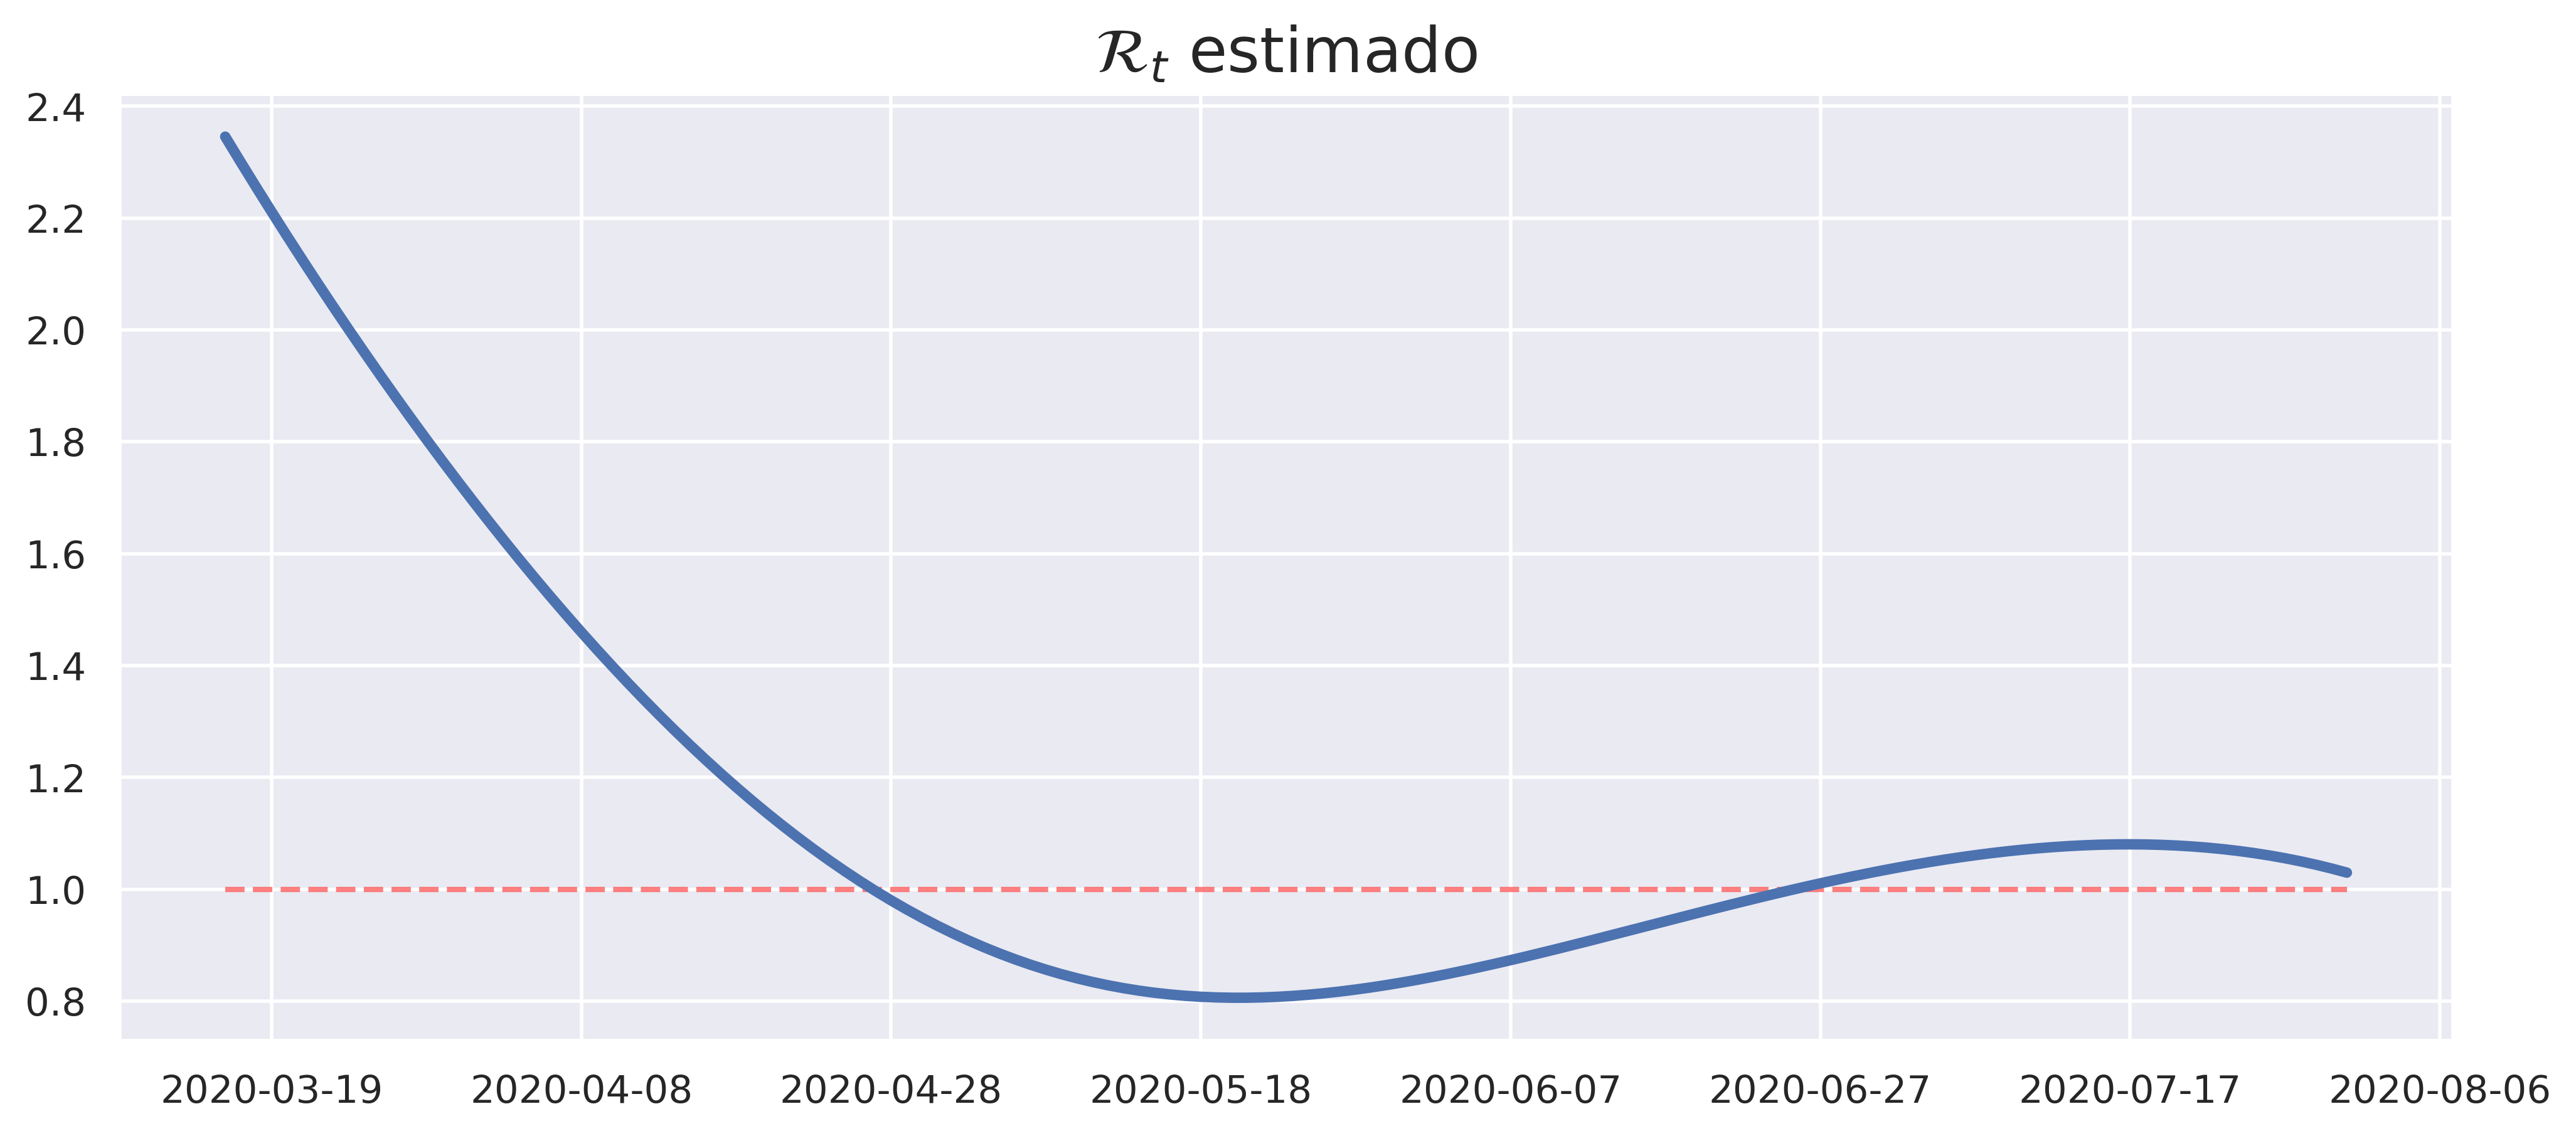
\includegraphics[width=0.8\textwidth]{../images/rt_example.png}
    \caption{Número reprodutivo ao longo do primeiros cinco meses de pandemia para os parâmetros do exemplo.}
    \label{Fig:rt_modelo}
\end{figure}

Para determinar a ordem $r$ e $s$, e o número de coeficientes para a aproximação por B-splines, usamos o {\em critério de informação AIC} descrito em \cite{liang2010}, que sob a hipótese de normalidade dos erros, pode ser calculado segundo a fórmula 
\begin{equation}
    AIC = n\ln\left(\frac{RSS}{n}\right) + 2K, 
\end{equation}
onde $K$ é o número de parâmetros desconhecidos e $RSS$ é a soma dos quadrados dos resíduos do modelo. Os resultados podem ser conferidos na Tabela \ref{Tab:aic-comparison}. 
Para esse experimento, escolhemos comparar modelos com 3 e 4 coeficientes, pois modelos com menos do que 3 coeficientes se mostrarem incapazes de capturar a variação temporal, enquanto modelos com mais do que 4 parâmetros são difíceis de estimar. 
Com isso, a ordem das splines pode variar de $k = 0$ a $k = \text{número de coeficientes} - 1$. 

\begin{table}[ht]
    \centering
    \begin{tabular}{|l|c|c|c|c|c|c|c|c|}
    \hline
    \multicolumn{2}{|c|}{\multirow{2}{*}{B-splines}}                       &
    \multicolumn{7}{|c|}{Parâmetros $\mu$}
    \\ \cline{3-9} 
    \multicolumn{2}{|c|}{}                                        & \textbf{(3,0)} & \textbf{(3,1)} & \textbf{(3,2)} & \textbf{(4,0)} & \textbf{(4,1)} & \textbf{(4,2)} & \textbf{(4,3)} \\ \hline
    \multirow{7}{*}{\rotatebox[origin=c]{90}{Parâmetros $\beta$}} & \textbf{(3,0)} & -2.021        & -2.029         & -2.023         & -2.025         & -2.028         & -2.032         & -2.001        \\ \cline{2-9} 
    & \textbf{(3,1)} & -2.228         & -2.241         & -2.266         & -2.288         & -2.298         & -2.311         & -2.298           \\ \cline{2-9} 
    & \textbf{(3,2)} & -2.246         & -2.230         & -2.253         & -2.294         & -2.337         & -2.331         & -2.309         \\ \cline{2-9} 
    & \textbf{(4,0)} & -1.967         & -1.979         & -1.979         & -1.998         & -2.002         & -2.000         & -1.987         \\ \cline{2-9} 
    & \textbf{(4,1)} & -2.262         & -2.304         & -2.277         & -2.302         & -2.372         & -2.348         & -2.338         \\ \cline{2-9} 
    & \textbf{(4,2)} & -2.346         & -2.243         & -2.262         & -2.300         & -2.374         & -2.357         & -2.332         \\ \cline{2-9} 
    & \textbf{(4,3)} & -2.213         & -2.233         & -2.251         & -2.294         & -2.363         & -2.347         & -2.323         \\ \hline
\end{tabular}
    \caption{Seleção de modelo segundo o AIC (escala $10^3$): os parâmetros que variam no
    tempo aproximados por 3 ou 4 parâmetros e ordem de 0 ao número
    de coeficientes - 1.}
    \label{Tab:aic-comparison}
\end{table}

Segundo o critério, o modelo escolhido possui 4 coeficientes para os dois parâmetros, com ordem das B-splines 2 para $\beta$ e 1 para $\mu$. 
Os resultados para o modelo escolhido não são muito diferentes dos gráficos já apresentados, incluindo a estimação de $\alpha = 0.898$ e podem ser conferidos no Github.

\subsubsection{Identificabilidade prática}
\label{identificability-practical}

O processo de identificabilidade estrutural desenvolvido na Seção \ref{identificability} é feito com base em duas hipóteses: a estrutura do modelo é precisa e os erros de mensuração são ausentes. 
Essas hipóteses não são válidas na prática e, por isso, é necessário avaliar se os parâmetros podem ser estimados de forma confiável e com precisão a partir dos dados ruidosos \cite{miao2011}. 
Seja $\hat{\theta} = (\hat{\alpha}, \hat{\beta}_1, ...,\hat{\mu}_{r})$ o vetor de estimativas a partir do ajuste aos dados. 
A {\em matriz de correlação} é um método que examina as correlação entre os parâmetros do modelo e pode ser calculada com base na {\em matriz Informação de Fisher (FIM)} da seguinte maneira, 
\begin{equation}
    FIM = \frac{1}{\hat{\sigma}_1^2}\left(\frac{\partial \hat{T}}{\partial \theta}\right)\Bigg|_{\theta = \hat{\theta}}^{T}\Sigma^{-1}\left(\frac{\partial \hat{T}}{\partial \theta}\right)\Bigg|_{\theta = \hat{\theta}} + \frac{1}{\hat{\sigma}_2^2}\left(\frac{\partial \hat{D}}{\partial \theta}\right)\Bigg|_{\theta = \hat{\theta}}^{T}\Sigma^{-1}\left(\frac{\partial \hat{D}}{\partial \theta}\right)\Bigg|_{\theta = \hat{\theta}}
    \label{fim}
\end{equation}
e a {\em matriz de covariâncias} $C$ é igual a inversa de $FIM$ (equação \eqref{fim}). Finalmente, o elemento $r_{ij}$, $1 \le i,j \le r + s + 1$ da {\em matriz de correlações} pode ser definido como 
\begin{equation}
    r_{ij} = \frac{C_{ij}}{\sqrt{C_{ii}C_{jj}}}
    \label{correlation}
\end{equation}
que mensura a correlação entre as estimativas $\hat{\theta}_i$ e $\hat{\theta}_j$. 
Uma correlação próxima a 1 indica que os parâmetros são praticamente indistinguíveis e um depende fortemente do outro. 
Em particular, ao calcularmos $R = [r_{ij}]$ para os parâmetros estimados, obtemos uma uma matriz de dimensão $K \times K$ onde $K$ é o número de parâmetros. 
Podemos visualizar através de um mapa de calor na Figura \ref{fig:corr-matrix} que $\alpha$ e o segundo coeficiente da B-spline de $\beta$ são fortemente correlacionados, mas negativamente. Isso não é um bom sinal quando se trata de identificabilidade.

\begin{figure}[!hb]
    \centering
    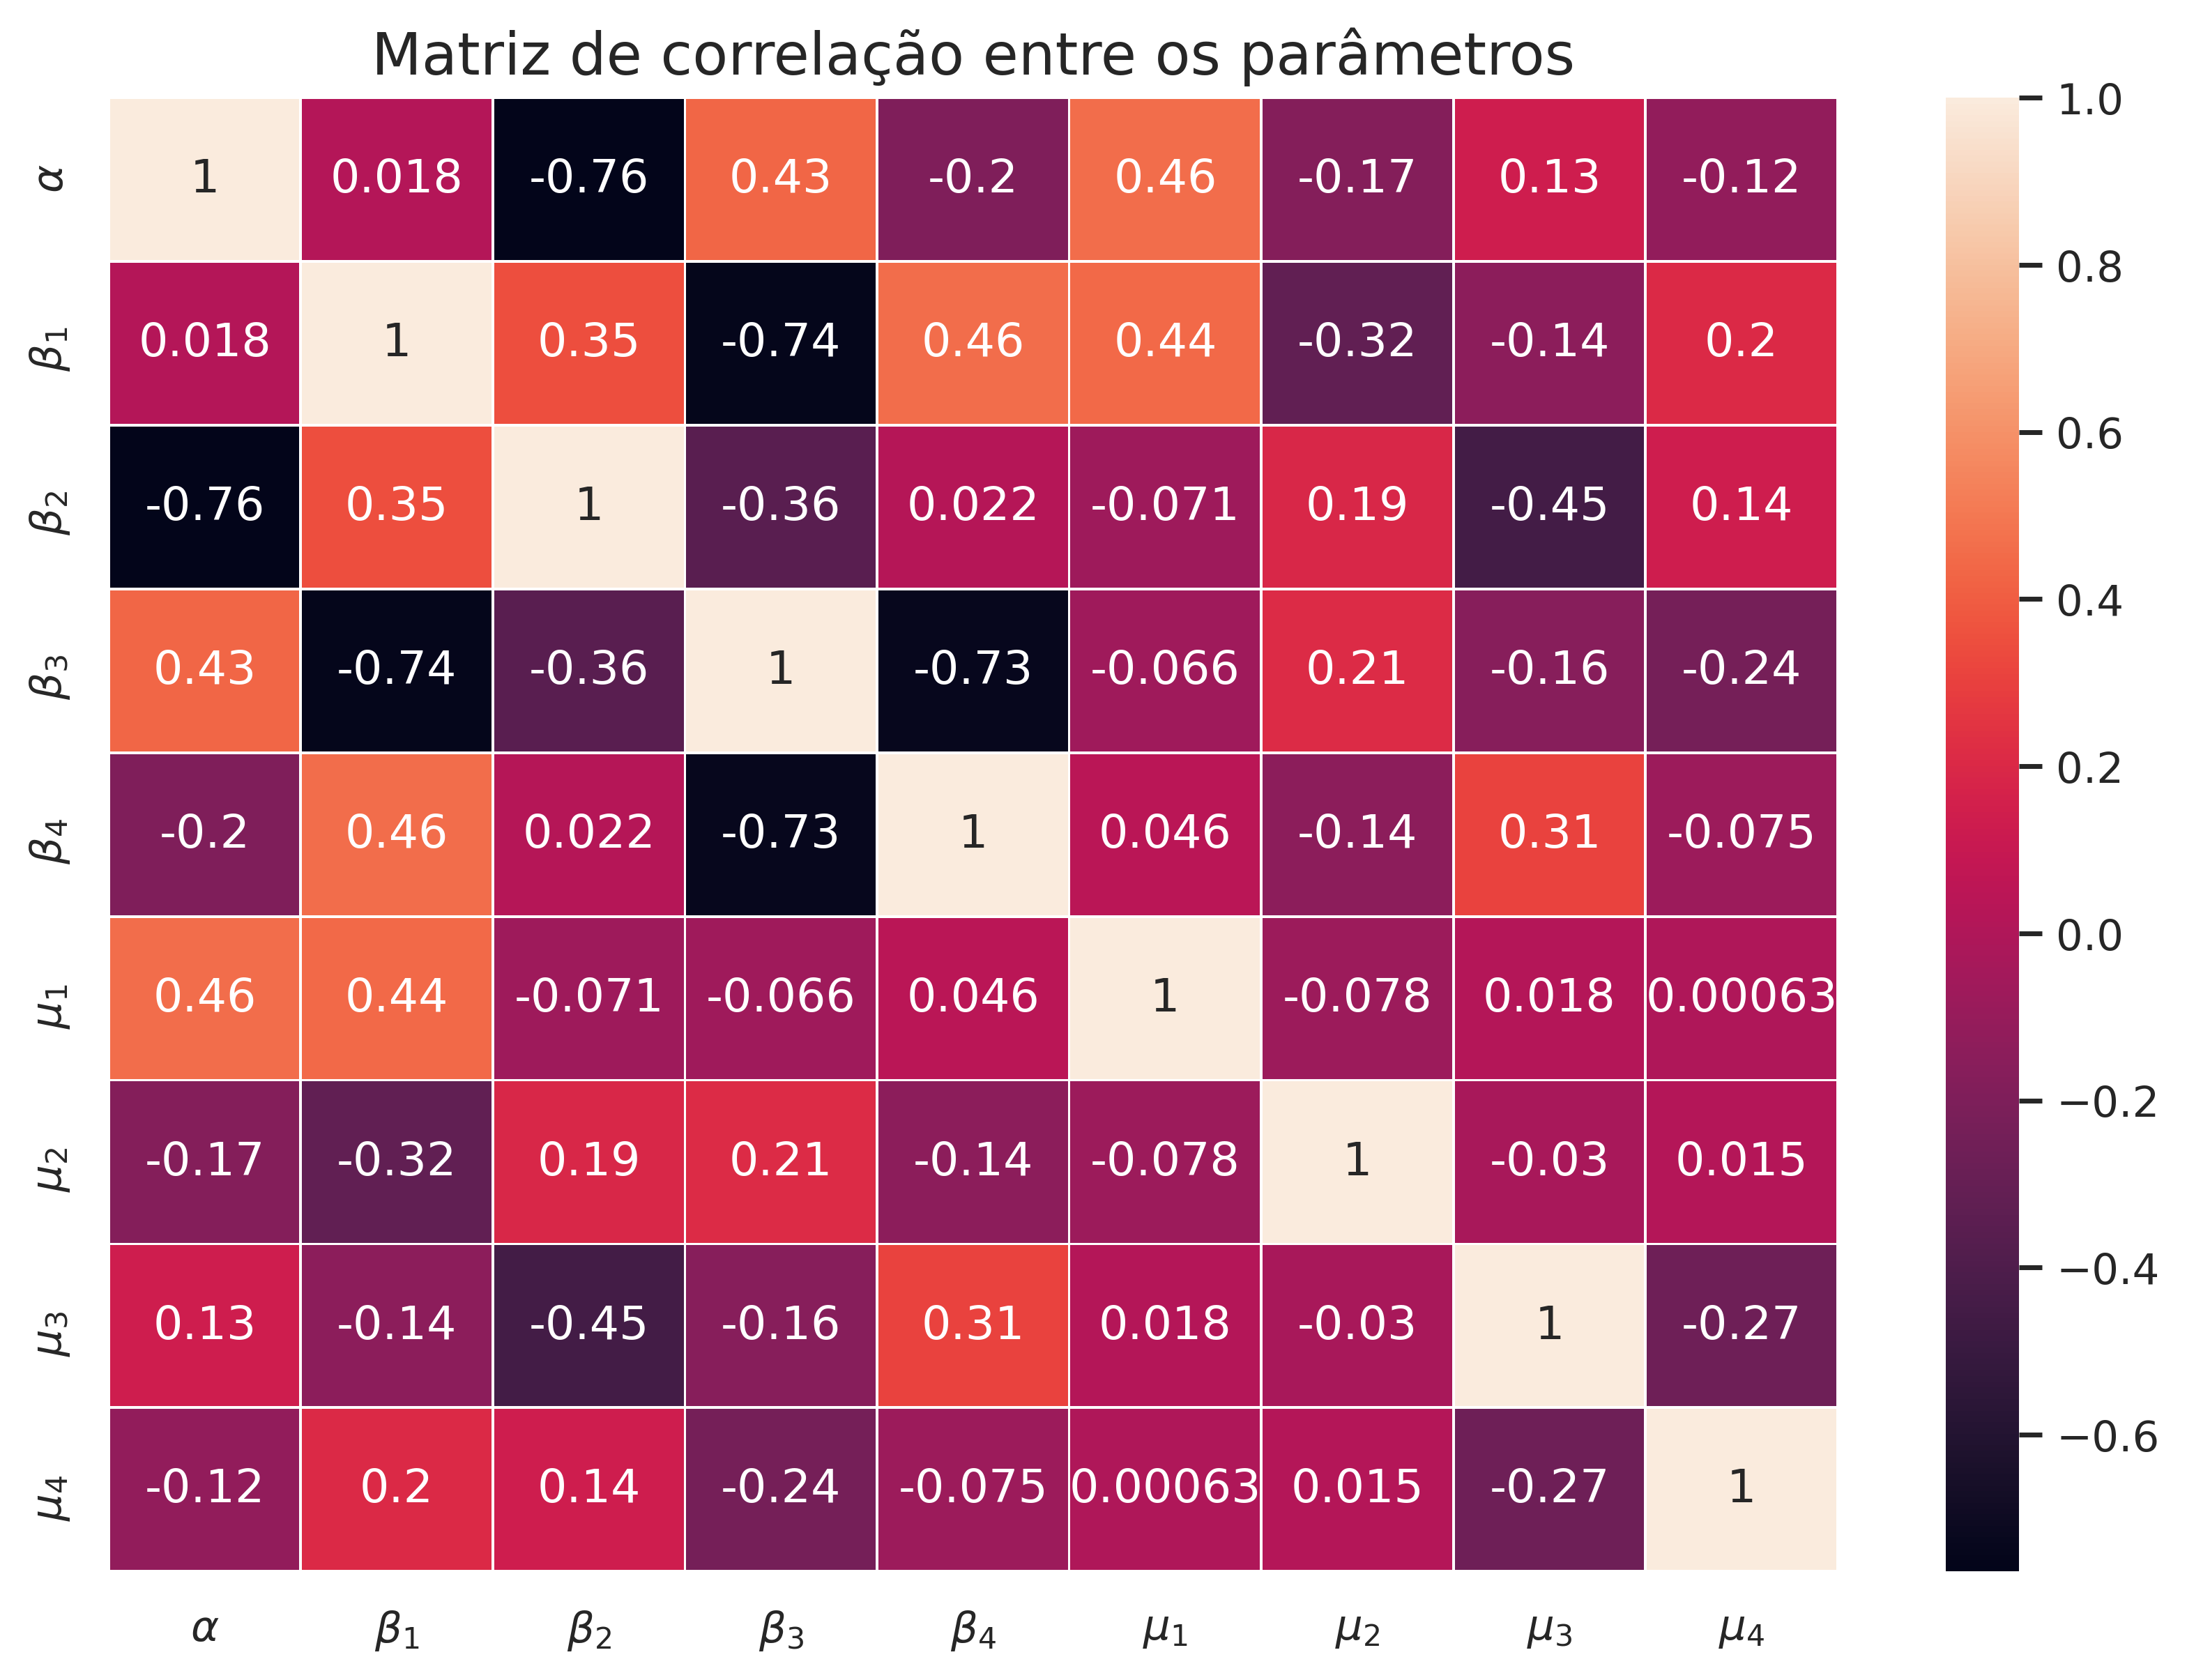
\includegraphics[width=0.8\textwidth]{../images/correlation_matrix.png}
    \caption{Matriz de correlação dos parâmetros estimados do modelo.}
    \label{fig:corr-matrix}
\end{figure}

Outra questão que pode ser levantada é sobre a influência da escolha dos parâmetros epidemiológicos, isto é, se eles variassem um pouco, o quanto isso afetaria a estimação de $\alpha$. 
Para fazer essa análise, escolhemos uma rede de valores para cada parâmetro baseada nos intervalos de confiança estimados nos respectivos artigos citados na Tabela \ref{tab:parameter_values}, estimamos os parâmetros do modelo e reportamos os menores intervalos que englobam os
valores estimados de $\alpha$ (com precisão até a terceira casa decimal), que podem ser conferidos na Tabela\ref{tab:range-parameters}. 
A fixação dos parâmetros influi pouco na estimação final de $\alpha$, portanto. 

\begin{table}[!hb]
    \centering
    \begin{tabular}{|c|c|c|}
    \hline
    \textbf{Parâmetro} & \textbf{Intervalo} & \textbf{Faixa de valores de $\alpha$} \\ \hline
    $\tau^{-1}$        & $[2,4]$            & $[0.897,0.902]$                       \\ \hline
    $\sigma^{-1}$      & $[2,4.5]$          & $[0.897, 0.9]$                         \\ \hline
    $\rho$             & $[0,10^{-4}]$      & $[0.898, 0.899]$                               \\ \hline
    $\gamma_1^{-1}$    & $[6.5,9.5]$        & $[0.894, 0.903]$                       \\ \hline
    $\gamma_2^{-1}$    & $[11,16]$          & $[0.896, 0.898]$                       \\ \hline
    \end{tabular}
    \caption{Rede de valores dos parâmetros fixados e o menor intervalo que inclui os valores estimados de $\alpha$}
    \label{tab:range-parameters}
\end{table}

\subsection{Quantificando incerteza sobre os parâmetros}

Os parâmetros estimados em um sistema dinâmico estão sujeitos à incerteza presente na captura dos dados, tal como erros de mensuração ou a variabilidade natural dos dados, e nas hipóteses adotadas pelo método de estimação. 
Assim, nessa seção, o objetivo será construir intervalos de confiança para os parâmetros desconhecidos de forma que, no longo prazo, a proporção dos intervalos calculados que contêm o parâmetro seja o nível desejado. 
Utilizaremos o {\em método Bootstrap} \cite{efron1986} que tem uma abordagem por simulação baseada nos dados. Ele gera, a partir de uma série $Y$, dados replicados $Y_1^*, ...., Y_N^*$ e realiza as estimações para cada um. 
Os intervalos de confiança para os valores de interesse são, então, os percentis correspondentes das $N$ amostras replicadas \cite{joshi2006}. 

Como consequência da estrutura dos erros apresentada nas equações \eqref{obsT1} e \eqref{obsD1}, as curvas são geradas com o valor inicial $\hat{T}(0) = y_0^{(1)}$ e para cada $i \ge 1$, $\hat{T}(i+1) = \hat{T}(i) + \varepsilon_{i+1}$, em que $\varepsilon_{i+1} \sim \mathcal{N}(\hat{x}_{i+1}^{1}, \hat{\sigma}_1^2)$ e $\hat{\sigma}_1^2$ é a estimativa para $\sigma_1^2$. A construção é análoga para a curva de óbitos.
Os parâmetros, então, foram estimados para cada uma das simulações. 
Além disso, para evitar que todas as simulações resultem em uma mesma região com mínimo locais, aleatorizamos o chute inicial do algoritmo de otimização. Para cada $j$ entre $1$ e $r+s+1$, $\theta_j^{inicial}$ é tomado aleatoriamente com distribuição uniforme no intervalo $(l_j, u_j)$, isto é, entre os limites inferior e superior estabelecidos. Realizamos esse processo $m$ vezes e tomamos a estimação com menor erro na função objetivo (equação \eqref{objective}). 

Fizemos $N = 500$ simulações com $m = 10$ (ou seja, $5000$ simulações no
total) e os outros parâmetros definidos como na Seção \ref{residual-analysis}. Após as simulações, estimamos os intervalos de confiança para os
parâmetros com nível 95\%, assim como as curvas $\mathcal{R}_t$ induzidas a
cada tempo $t$. O intervalo estimado para a taxa de subnotificação $\alpha$
foi $(0.849,0.931)$. Na Figura \ref{fig:rt-confidence-interval}, é possível
visualizar os intervalos de $\mathcal{R}_t$. É interessante visualizar o
gráfico que exibe as relações dois a dois entre os parâmetros, o que mostra a
correlação nas estimações. 
As correlações estimadas na Figura \ref{fig:corr-matrix} podem ser observadas
nos gráficos de dispersão na Figura \ref{fig:correlation-bootstrap}, como, por
exemplo, a relação linear entre $\alpha$ e $\beta_2$. 
Os histogramas dos parâmetros também podem ser observados. Na Tabela \ref{tab:bootstrap-estimations} é sumarizada a informação para todos os parâmetros. Informações e gráficos adicionais podem ser visualizados no Github \cite{github}.

\begin{figure}
    \centering
    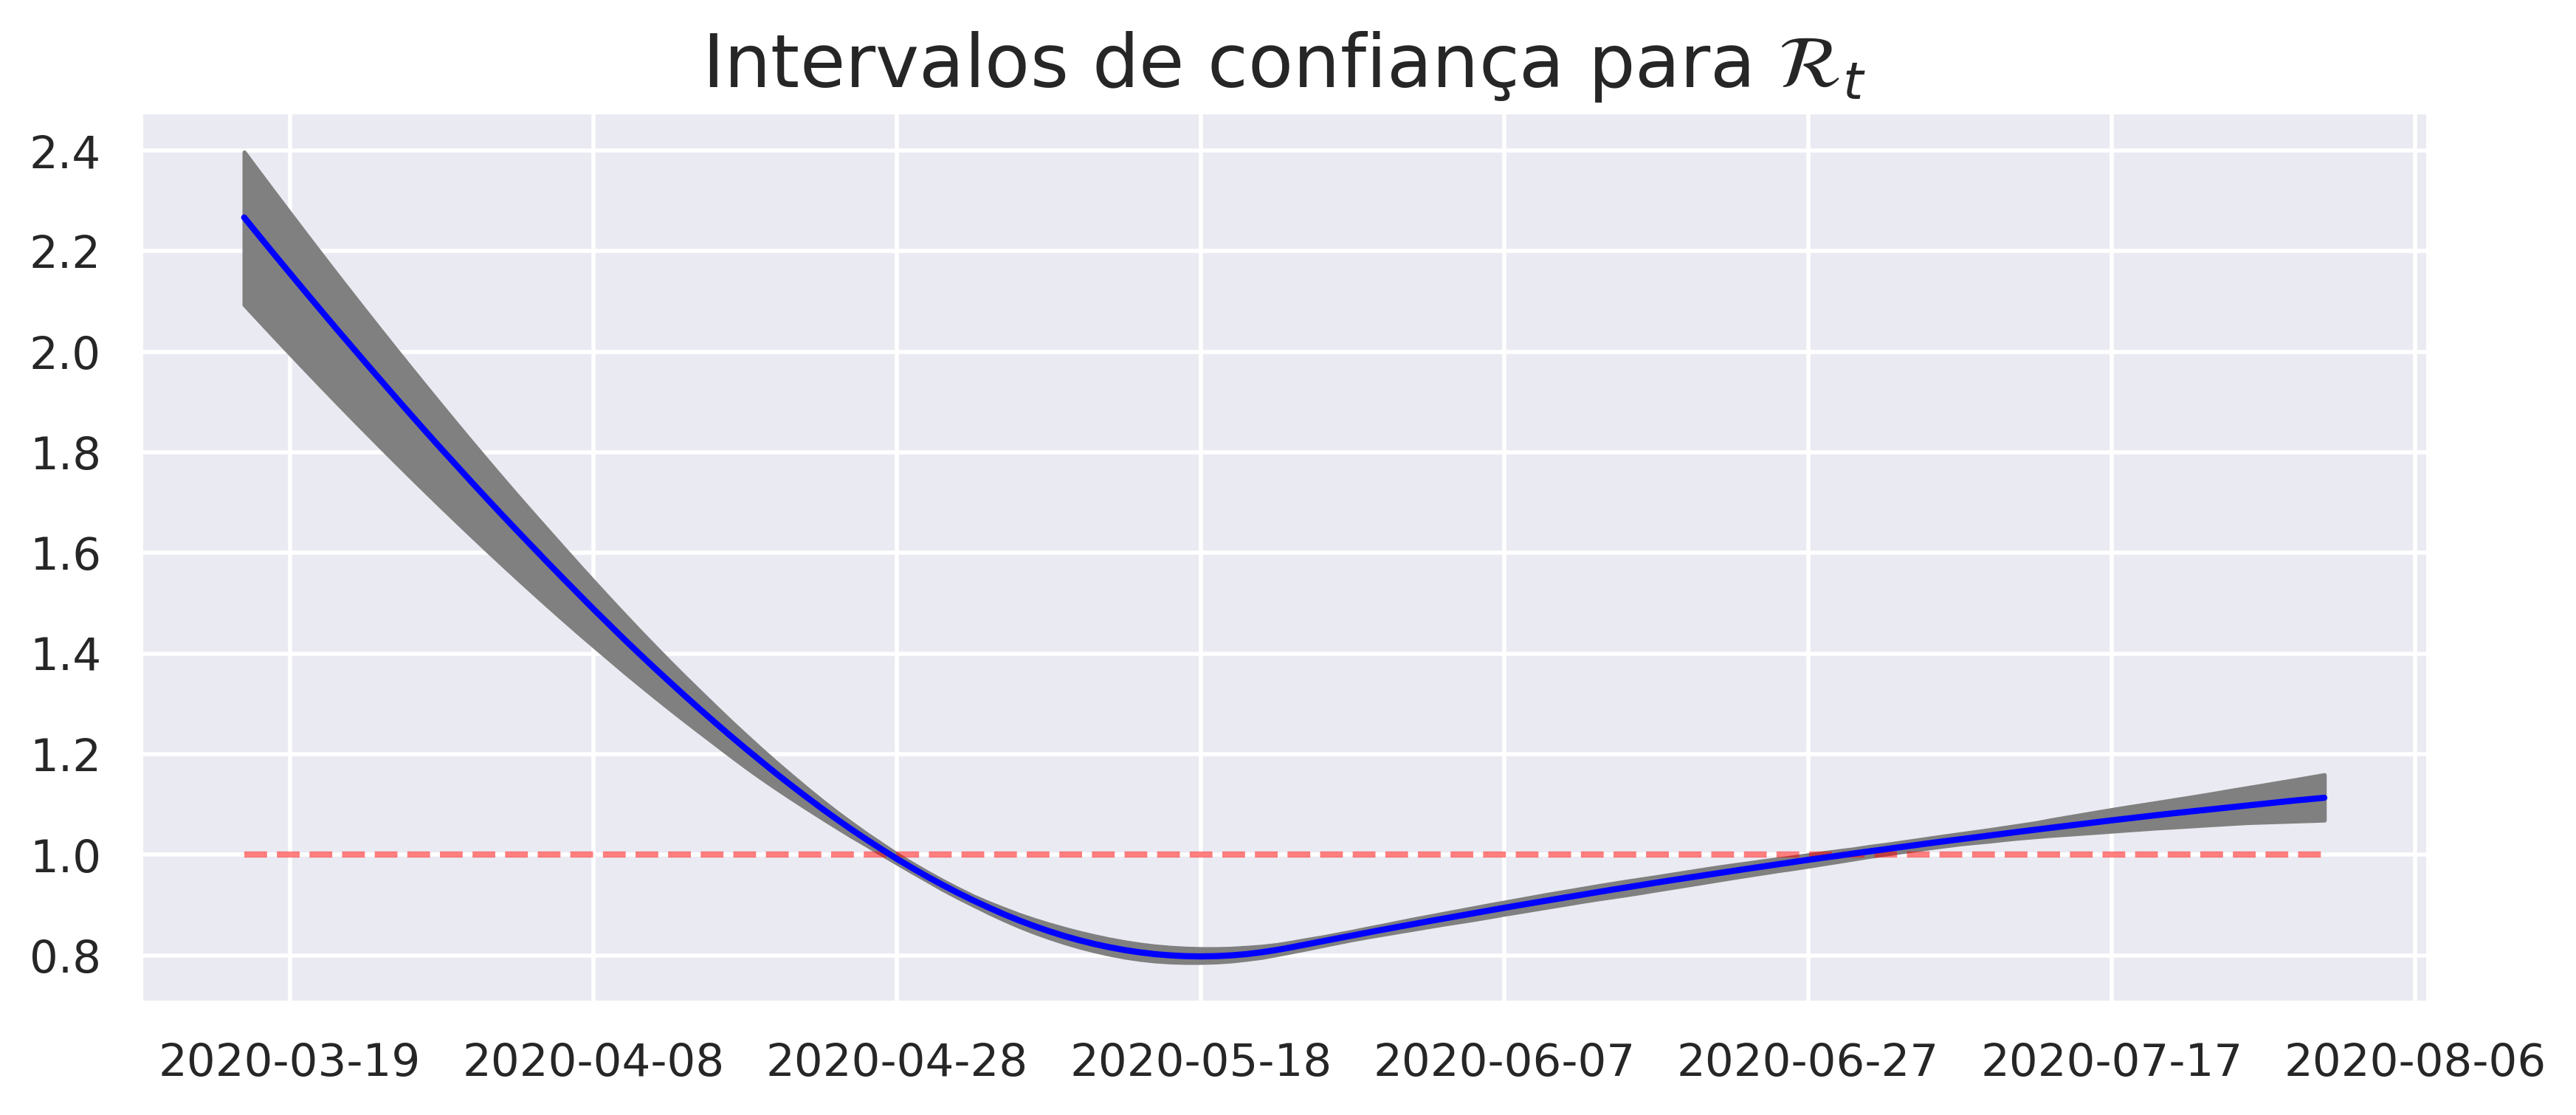
\includegraphics[width = 0.9\textwidth]{../images/rt_confidence_interval.png}
    \caption{A curva em azul é a mediana das curvas estimadas e em cinza o
    intervalo de confiança. Em vermelho é o limiar 1 para o $\mathcal{R}_t$.}
    \label{fig:rt-confidence-interval}
\end{figure}

\begin{figure}
    \centering
    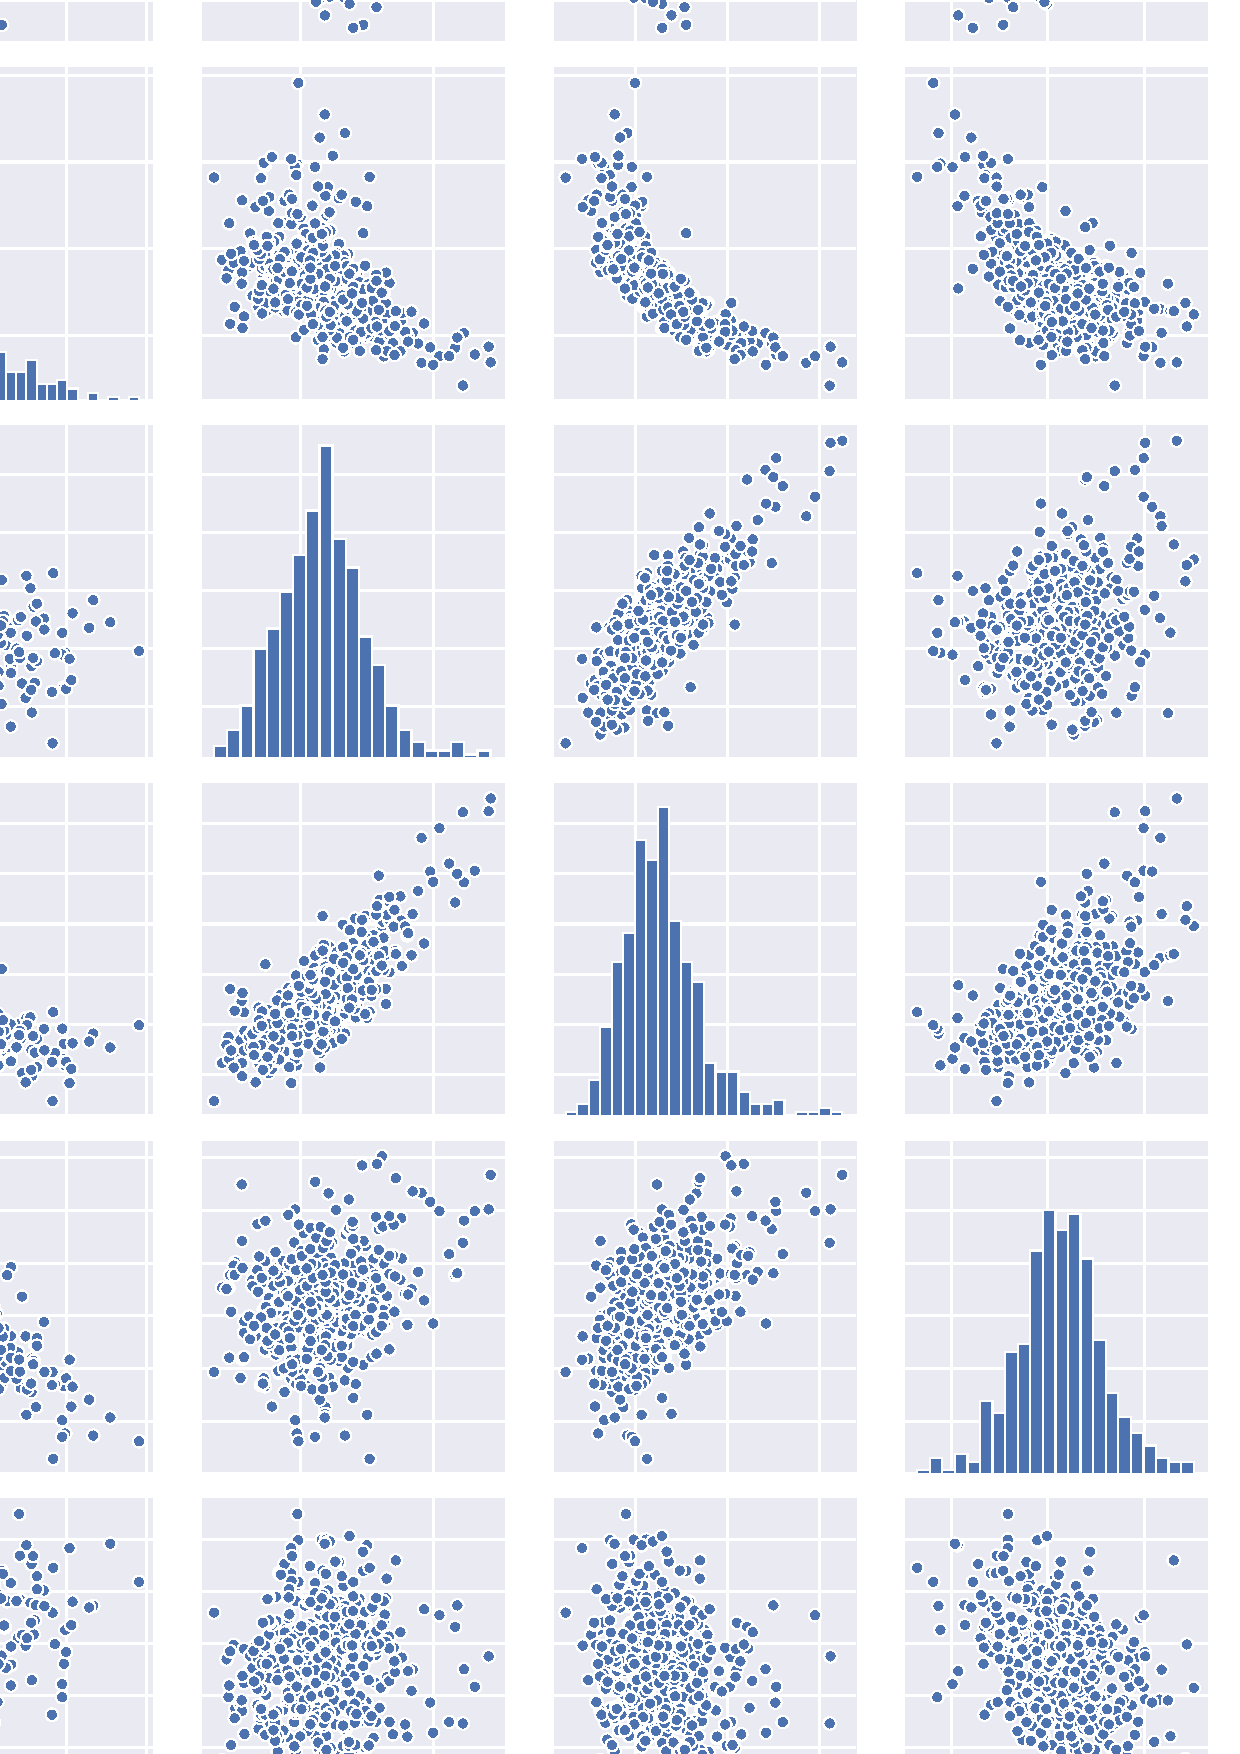
\includegraphics[width = \textwidth]{../images/correlation_bootstrap.png}
    \caption{Gráficos de dispersão a cada dois parâmetros indicando a relação entre eles e os histogramas das estimativas.}
    \label{fig:correlation-bootstrap}
\end{figure}

\begin{table}[!ht]
    \centering
    \begin{tabular}{|c|c|c|}
    \hline
    \textbf{Parâmetro} & \textbf{Mediana} & \textbf{Intervalo calculado} \\ \hline
    $\alpha$        & $0.903$            & $[0.849,0.93]$                      \\ \hline
    $\beta_1$      & $0.144$          & $[0.142, 0.147]$                        \\ \hline
    $\beta_2$      & $0.073$          & $[0.069, 0.079]$                        \\ \hline
    $\beta_3$      & $0.101$          & $[0.098, 0.104]$                        \\ \hline
    $\beta_4$      & $0.126$          & $[0.123, 0.132]$                        \\ \hline
    $\mu_1$    & $0.0101$        & $[0.0092, 0.011]$                       
    \\ \hline
    $\mu_2$    & $0.0159$        & $[0.0154, 0.0164]$               
    \\ \hline
    $\mu_3$    & $0.0103$        & $[0.0098, 0.0108]$                       
    \\ \hline
    $\mu_4$    & $7.03\cdot 10^{-3}$        & $[6.73\cdot 10^{-3}, 7.38\cdot 10^{-3}]$                       
    \\ \hline
    \end{tabular}
    \caption{Estimativas da mediana e dos intervalos de confiança para cada parâmetro desconhecido do modelo.}
    \label{tab:bootstrap-estimations}
\end{table}

\section{Conclusão}
\label{conclusion}

Nesse trabalho, utilizamos ferramentas matemáticas de equações diferenciais,
estatística e otimização para estimar a taxa subnotificação de COVID-19 na
cidade do Rio de Janeiro no início da pandemia. Obtivemos que a proporção
$\alpha$ de indivíduos não identificados pelo sistema é em torno de 90\%, com
intervalo de confiança entre 85\% e 92\%. Isso significa que a cada indivíduo
notificado pelo sistema, em torno de 9 ou 10 não foram observados, por serem 
assintomáticos, apresentarem sintomas leves ou não serem testados. Esse valor
está de encontro com várias cidades do Brasil, de acordo com
\cite{subnotificacao-folha-de-sao-paulo}. Em uma nota técnica de abril de 2020,
\cite{subnotification-brazil} estimou a notificação de casos no Brasil entre
7.8\% e 8.1\% e \cite{subnotification2-brazil}, também em abril de 2020, em
7\%. No Rio de Janeiro, \cite{subnotification-rio} estimou a notificação em
7.2\%. Esses resultados vão de encontro com o desse trabalho. 

A análise de dados na Seção \ref{data} permitiu o melhor entendimento de
problemas em relação ao tempo de notificação de um indivíduo infectado. Nesse
sentido, além da falta de testagem, existem atrasos e erros em todas as etapas do
processo que, sem o devido cuidado, podem gerar más inferências.
Gráficos adicionais sobre as outras variáveis estão em formato {\it notebook}
no Github \cite{github}. Obtivemos um ajuste interessante do modelo, com
resíduos distribuídos normalmente, apesar de estarem correlacionados. Os
resultados de identificabilidade estrutural (Seção \ref{identificability}) reforçam a necessidade da obtenção
da curva de recuperados, enquanto na identificabilidade prática (Seção \ref{identificability-practical}),
sugerem que outra abordagem para estimar as curvas de transmissibilidade e
mortalidade deve ser tomada. A despeito disso, a adoção de limites nos parâmetros permitiu
uma estimação mais precisa, inclusive quando os parâmetros previamente fixados
variavam (ver Tabela \ref{tab:range-parameters}). 

O número reprodutivo básico como função do tempo mostrou ter um comportamento
similar às outras estimativas, como mencionado em \ref{residual-analysis}. A
pouca variabilidade deve-se à suavidade induzida pelas B-splines. Para
construir uma curva mais suscetível a mudanças diárias, uma aproximação por
outro método deve ser adotada. Por fim, a aparente subestimação da incerteza
nessa curva deriva dessa problemática. Outras fontes de incerteza podem ser
adicionadas ao Bootstrap em trabalhos futuros. 

\section{Agradecimentos}

Gostaria de agradecer à Orientadora do trabalho Maria Soledad Aronna
(FGV/EMAp, Rio de Janeiro) pela
compreensão e aconselhamento ao longo do processo. Agradecer também aos
professores Roberto Guglielmi (Universidade de Waterloo, Canadá) e Luiz Max de
Carvalho (FGV/EMAp, Rio de Janeiro) pela contribuição em
tópicos importantes. Essa iniciação científica foi apoiada pela FAPERJ
(Brasil) através do Programa ``Jovem Cientista do Nosso Estado'' e pelo CNPq
(Brasil) através do Programa ``Iniciação Científica e Mestrado'' (PICME). 

\begin{thebibliography}{00}

\bibitem{audoly2001}
Audoly, S. {\it et al}. Global identifiability of nonlinear models of biological
systems.{\it IEEE Transactions on Biomedical Engineering} 48(1):55-65, 2001, DOI: 10.1109/10.900248.

\bibitem{aronna2021}
Aronna, M. S., Guglielmi, R., Moschen, L. M. A model for COVID-19 with
isolation, quarantine and testing as control measures. {\it Epidemics}. 34,
2021. DOI: 10.1016/j.epidem.2021.100437

\bibitem{rtBrasil2020}
Bastos, S. B., Cajueiro, D. O. Modeling and forecasting the early evolution of
the covid-19 pandemic in brazil. {\it Scientific Reports}, 10(1):19457, 2020.
DOI: 10.1038/s41598-020-76257-1.

\bibitem{bellu2007}
Bellu, G., Saccomani, M. P., Audoly, S., D'Angiò, L. DAISY: a new software
tool to test global identifiability of biological and physiological systems.
{\it Comput Methods Programs Biomed}. 88(1):52-61, 2007.
DOI:10.1016/j.cmpb.2007.07.002.

\bibitem{byrd1995}
Byrd, R. H., Lu P., Nocedal, J., Zhu, C. A Limited Memory Algorithm for Bound
Constrained Optimization. {\it SIAM Journal on Scientific and Statistical
Computing} 16(5): 1190-1208, 1995. DOI: 10.1137/0916069

\bibitem{recovery2020}
Byrne A. W. {\it et al}. Inferred duration of infectious period of SARS-CoV-2:
rapid scoping review and analysis of available evidence for asymptomatic and
symptomatic COVID-19 cases. {\it BMJ Open}. 10(8), 2020. DOI: 10.1136/bmjopen-2020-039856.

\bibitem{subnotificacao-folha-de-sao-paulo}
Canzian, F. Estados e municípios no país relatam subnotificação gigantesca de casos. {\it Folha de São Paulo}. \url{https://www1.folha.uol.com.br/equilibrioesaude/2020/04/estados-e-municipios-no-pais-relatam-subnotificacao-gigantesca-de-casos.shtml}, abril de 2020. 

\bibitem{cao2012}
Cao, J., Huang J. Z., Wu H. Penalized Nonlinear Least Squares Estimation of Time-Varying Parameters in Ordinary Differential Equations. 
{\it Journal of Computational and Graphical Statistics}, 21:1, 42-56, 2012.
DOI: 10.1198/jcgs.2011.10021

\bibitem{croda2020}
Croda, J. {\it et al}. COVID-19 in Brazil: advantages of a socialized unified health
system and preparation to contain cases. {\it Rev. Soc. Bras. Med. Trop.} 53,
2020. DOI: 10.1590/0037-8682-0167-2020

\bibitem{dantas2020}
Dantas, G. {\it et al}. The impact of COVID-19 partial lockdown on the air quality
of the city of Rio de Janeiro, Brazil. {\it Science of The Total Environment},
729, 2020. DOI: 10.1016/j.scitotenv.2020.139085.

\bibitem{efron1986}
Efron, B., Tibshirani, R. Bootstrap Methods for Standard Errors, Confidence
Intervals, and Other Measures of Statistical Accuracy. {\it Statist. Sci.}
1(1):54-75, 1986. DOI: 10.1214/ss/1177013815

\bibitem{sistemas-bandeiras}
Estadão. Governo do Rio cria classificação em 3 bandeiras para flexibilizar isolamento. \url{https://revistapegn.globo.com/Noticias/noticia/2020/05/pegn-governo-do-rio-cria-classificacao-em-3-bandeiras-para-flexibilizar-isolamento.html}, maio de 2020.

\bibitem{ibge-pnad}
IBGE – Instituto Brasileiro de Geografia e Estatística. Pesquisa Nacional por
Amostra de Domicílios - PNAD COVID19.
\url{https://www.ibge.gov.br/estatisticas/sociais/trabalho/27946-divulgacao-semanal-pnadcovid1.html?=&t=downloads}.
2020.

\bibitem{ibge-rio}
IBGE – Instituto Brasileiro de Geografia e Estatística. Cidades e Estados.
\url{https://www.ibge.gov.br/cidades-e-estados/rj/rio-de-janeiro.html}.
2021.

\bibitem{jarque1980}
Jarque, C. M., Bera, A. K. Efficient tests for normality, homoscedasticity and serial independence of regression residuals.
{\it Economics Letters}, 6(3): 255-259, 1980. DOI:
10.1016/0165-1765(80)90024-5

\bibitem{joshi2006}
Joshi, M., Seidel-Morgenstern, A. Kremling, A. Exploiting the bootstrap method
for quantifying parameter confidence intervals in dynamical systems. {\it
Metabolic Engineering}, 8(5): 447-455, 2006. DOI: 10.1016/j.ymben.2006.04.003

\bibitem{delta2020}
Kucirka L. M. {\it et al}. Variation in
false-negative rate of reverse transcriptase polymerase chain reactionbased
SARS-CoV-2 tests by time since exposure. {\it Ann Intern Med}. 173(4):262–7,
2020. DOI: 10.7326/M20-1495

\bibitem{latent2020}
Li R, Pei S, Chen B, {\it et al}. Substantial undocumented infection
facilitates the rapid dissemination of novel coronavirus (SARS-CoV-2). {\it Science}.
368(6490):489-493, 2020. DOI:10.1126/science.abb3221

\bibitem{liang2010}
Liang, H., Miao, H., Wu, H. Estimation of constant and time-varying dynamic parameters of HIV infection in a nonlinear differential equation model. {\it Ann. Appl. Stat. 4}, 1: 460-483, 2010. DOI 10.1214/09-AOAS290

\bibitem{ljung1978}
Ljung, G. M., Box, G. E. P. On a measure of lack of fit in time series models.
{\it Biometrika}, 65:297-303, 1978. DOI: 10.1093/biomet/65.2.297

\bibitem{ljung1994}
Ljung, L. , Glad, T. On global identifiability for arbitrary model
parametrizations. {\it Automatica}, 30: 265-276, 1994.
DOI:10.1016/0005-1098(94)90029-9.

\bibitem{rt-imperial-college}
Mellan, T., {\it et al.} Subnational analysis of the COVID-19 epidemic in
Brazil. {\it Cold Spring Harbor Laboratory Press}, 2020. DOI:
10.1101/2020.05.09.20096701. 

\bibitem{miao2011}
Miao, H., Xia, X. Perelson, A. S., Wu, H. On Identifiability of Nonlinear ODE Models and Applications in Viral Dynamics.
{\it SIAM Review}, 53(1): 3-39, 2011. DOI: 10.1137/090757009

\bibitem{github}
Moschen, L. M. Repositório Covid-19. {\it Github}. Disponível em \url{https://github.com/lucasmoschen/covid-19-model}.

\bibitem{nogrady}
Nogrady, B. What the data say about asymptomatic COVID infections. {\it
Nature}. 587: 534-535, 2020. DOI: 10.1038/d41586-020-03141-3

\bibitem{observatorio}
Observatório COVID-19 BR. R efetivo no Rio de Janeiro. Disponível em
\url{https://covid19br.github.io/municipios.html?aba=aba3&uf=RJ&mun=Rio_de_Janeiro}.
Acesso em abril de 2021. 

\bibitem{subnotification2-brazil}
Portal COVID-19 Brasil. COVID-19 BRASIL [acessado 2021 Abril]. Disponível em: \url{https://ciis.fmrp.usp.br/covid19/}

\bibitem{subnotification-brazil}
Prado, M. F. do {\it et al.} Análise de subnotificação do número de casos confirmados da COVID-19 no
Brasil. Disponível em
\url{https://drive.google.com/file/d/1_whlqZnGgvqHuWCG4-JyiL2X9WXpZAe3/view}. 

\bibitem{subnotification-rio}
Prado, M. F. do {\it et al}. Análise da subnotificação de COVID-19 no Brasil.
{\it Rev. bras. ter. intensiva [online]}. 32(2): 224-228, 2020. DOI: 10.5935/0103-507x.20200030.


\bibitem{incubation2020}
Rai, B., Shukla, A., Dwivedi, L.K. Incubation period for COVID-19: a
systematic review and meta-analysis. {\it J Public Health (Berl.)} 2021. DOI: 10.1007/s10389-021-01478-1

\bibitem{ramsey2007} 
Ramsay, J. O., Hooker, G., Campbell, D. e Cao, J. Parameter estimation for
differential equations: a generalized smoothing approach. {\it Journal of the
Royal Statistical Society: Series B (Statistical Methodology)}, 69:741--796,
2007. DOI:10.1111/j.1467-9868.2007.00610.x

\bibitem{decreto-emergencia}
Rio de Janeiro. Decreto nº 46.973, 16 de março de 2020. Reconhece a situação de emergência na saúde pública do estado do Rio de Janeiro em razão do contágio e adota medidas de enfrentamento da propagação decorrente do novo coronavírus (COVID-19); e dá outras previdências. {\bf Diário Oficial do Estado do Rio de Janeiro}, Rio de Janeiro, RJ, n. 049-A, 17 de março de 2020. Disponível em \url{https://pge.rj.gov.br/comum/code/MostrarArquivo.php?C=MTAyMjI}. 

\bibitem{decreto-mascaras}
Rio de Janeiro. Lei nº 8859, 03 de junho de 2020. Estabelece a obrigatoriedade do uso de máscaras respiratórias, no âmbito do estado do Rio de Janeiro, enquanto vigorar o estado de calamidade pública em virtude da pandemia do novo coronavírus (COVID-19). {\bf Diário Oficial do Estado do Rio de Janeiro}, Rio de Janeiro, RJ, n. 100, 04 de junho de 2020. Disponível em \url{http://www.aeerj.net.br/file/04-06-2020-leiestadomascara.pdf}. 

\bibitem{rodriguez2006}
Rodriguez-Fernandez, M., Egea, J. A., Banga, J. R. Novel metaheuristic for parameter estimation in nonlinear dynamic biological systems. {\it BMC Bioinformatics} 7:483, 2006. DOI: 10.1186/1471-2105-7-483

\bibitem{sarcomani2019}
Saccomani M. P., Thomaseth K. Calculating all multiple parameter solutions of
ODE models to avoid biological misinterpretations.{\it Mathematical
Biosciences and Engineering : MBE }, 16(6):6438-6453, 2019. DOI:
10.3934/mbe.2019322.

\bibitem{data-rio-covid}
Secretaria Municipal de Saúde (SMS), Prefeitura da Cidade do Rio de Janeiro. Dados individuais dos casos confirmados de COVID-19 no município do Rio de Janeiro. \url{https://www.arcgis.com/home/item.html?id=f314453b3a55434ea8c8e8caaa2d8db5}, março de 2021.

\bibitem{painel-rio-covid}
Secretaria Municipal de Saúde (SMS), Prefeitura da Cidade do Rio de Janeiro. Painel Rio COVID-19.\url{https://experience.arcgis.com/experience/38efc69787a346959c931568bd9e2cc4}, 2021.

\bibitem{sars-cov-2}
The 2019 nCoV Outbreak Joint Field Epidemiology Investigation Team and Q. Li.
An Out-break of NCIP (2019-nCoV) Infection in China - Wuhan, Hubei Province,
2019 -
2020.-\url{http://weekly.chinacdc.cn/en/article/id/e3c63ca9-dedb-4fb6-9c1c-d057adb77b57},
janeiro de 2020

\bibitem{scipy}
Virtanen P. {\it et al}. SciPy 1.0: Fundamental Algorithms for Scientific Computing
in Python. {\it Nature Methods}. 17(3): 261-272, 2020. 

\bibitem{oms-symptoms}
World Health Organization. Coronavirus disease (COVID-19).
\url{https://www.who.int/emergencies/diseases/novel-coronavirus-2019/question-and-answers-hub/q-a-detail/coronavirus-disease-covid-19#:~:text=symptoms},
outubro de 2020

\end{thebibliography}

\end{document}

